\documentclass[thesis_msc.tex]{subfiles}

\begin{document}

\chapter{Introduction} \label{intro}
 
     \paragraph{} In this chapter the history of pulsars will be briefly discussed. I will describe the formation of pulsars and the model to describe them. Then, I will introduce the effect of the interstellar medium (ISM) on electromagnetic waves. Applications of pulsars as physics tools will be briefly discussed here. 


    \section{What are Pulsars?}
    \paragraph{} In 1967, Antony Hewish and Jocelyn Bell discovered radio pulsations from the sky with a period of 1.34s \citep{HEWISH1968}. They identified them as an extraterrestrial source because of its fixed position in equatorial coordinates.  After discoveries of similar sources from the sky, the word pulsar (from pulsating star) is used to describe these objects. The maximum size of pulsars is approximated from light travel time across the pulsed emission \citep{HEWISH1968} need to be shorter than light travel time across the object. As a result, the short rotation period of pulsar leads to the deduction that this object has to be relatively small. Pulsars were hypothesised to be either rotating neutron stars (NS) or white dwarfs (WD). Both NS and WD are remnants of stars which collapsed into compact objects. \cite{PhysRev.46.76.2} proposed the pulsating NS theory was proposed despite no evidence on this object until the discovery of pulsars. After that, \cite{PACINI1967} and \cite{GOLD1968} confirmed that pulsars are rotating NS by the discovery of Crab pulsar because it located in supernova remnants \textit{Crab nebular}  with a period of 33 ms. Short period and the location in supernova remnants make us understand that Crab pulsar is associated with neutron star which is the last process of an intermediate mass star (See more in Section ~\ref{formation}) . Moreover, the short period indicates that this object needs to be more massive than WD (More detailed can be found in \cite{GOLD1968}).   
               
    \paragraph{} 50 years after the discovery of pulsars. The number of confirmed pulsar detection in June 2018 is approximately 2600 \citep{PSRCAT2}, and the up to date number can be found from http://www.atnf.csiro.au/people/pulsar/psrcat. Some significant milestones of pulsar astronomy are listed below.

\begin{itemize}
\item In 1934 Walter Baade and Fritz Zwicky proposed that dense stars consist of purely of neutrons could be a result from supernovae  ~\citep{baade1934remarks}.  

\item Discovery of the first pulsars in 1967 \citep{HEWISH1968}.

\item Franco Pacini suggested that neutron stars radiates electromagnetic waves in 1967 ~\citep{PACINI1967}. 

\item The discovery of the first pulsar gave  Antony Hewish a share of 1974 Nobel Prize in Physics \citep{HEWISH1968} with Sir Martin Ryle for his contribution on the discovery of NS.

\item The discovery of Hulse-Taylor pulsar PSR B1913+16 in 1974. This system is ``the first experimental demonstration of the existence of gravitational waves (GW)'' ~\citep{handbook} and earned them the 1993 Nobel Prize in Physics \citep{hulse1975discovery}.

\item The first pulsar which has rotation period in the order of millisecond  (B1937+21) with a period of 1.56 ms ~\citep{backer1982millisecond}. 

\item The discovery of the first ``Double pulsar'' system ~\citep{burgay2003increased}. This system consists of two pulsars. These pulsar allows us to make better constraints on strong-field gravitational theory ~\citep{lyne2004double}.

\item The discovery of the first magnetar ~\citep{usov1996persistent} in 1996. Further detail about magnetars can be found at Section ~\ref{magnetar}

\item The discovery of the Galactic centre magnetar J1745-2900 located near the galactic centre ~\citep{kennea2013swift}. This is the first time that astronomers can probe the environment around the galactic centre with a pulsar.  

\end{itemize}

    \section{Formation of Neutron stars} \label{formation}
    \paragraph{} After stars cannot sustain the balance between inward gravity force and outward force from radiation pressure originated from internal nuclear fusion. The stars will collapse into one of three kinds of astrophysical objects depends on the initial mass of the star. Low mass stars (M \textless 8 $M_\odot$) like our sun will collapse to WDs. WDs are compact objects compose by electron-degenerate matter. This matter producing outwards force prevent WDs from collapsing (\cite{WDNSBH} and \cite{d1997evolution}). Massive stars (M $>$ 25 $M_\odot$) will end up as black holes (BH). NSs are remnants from core collapsing of intermediate mass stars. The term ``intermediate'' here means 8-25 solar mass ($M_\odot$). Furthermore detailed about NS and BH evolution can be found at \cite{heger2003massive}

    \paragraph{} After an intermediate-mass star converted Hydrogen into Helium in its core, the thermonuclear fusion process will decreases while the mass of the star considers being almost the same from the beginning of their life. The gravitational force makes the Helium core contract until the temperature increases enough to make Helium nuclear fusion. This process continues for all the lifetime of the star producing more massive element and binding energy from the left side of Figure ~\ref{binding} toward the right side of the same figure. The last element that intermediate-mass produces from nuclear fusion is the Iron because its has the highest binding energy in Figure \ref{binding} while. After this point, the star could not further produce energy because fusion process requires more energy than they can produce \citep{burbidge1957synthesis} and decreeing their radiation pressure. The core will collapse while the outer layer is blown away called supernova remnant. The process of core contract makes a supernova explosion (to be specific for NS formation, Type II supernova). This collapse core has mass enough to beat electron degeneracy pressure that prevents WD from collapsing. The final stage of this process converts the iron core into a nuclear matter which mainly consists of neutrons. Furthermore, detail about NS formation can be found at ~\citep{cameron1969neutron} and ~\citep{portegies1998formation}. 

    \begin{figure}[h] \centering
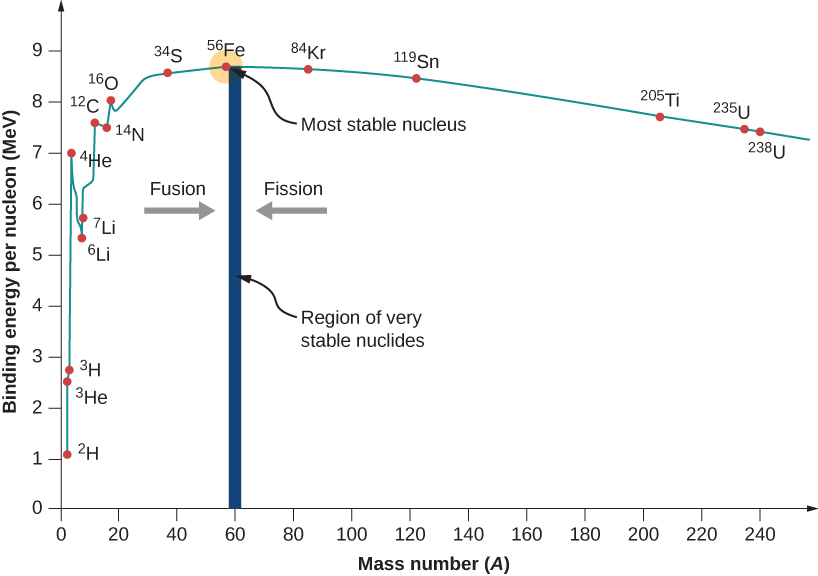
\includegraphics[width=0.70\textwidth]{figures/binding.jpg}
\caption{Relation between binding energy and mass number shows peaks at Iron, which make Iron the most stable element. Image from \cite{urone_hinrichs_dirks_sharma_2018} }

\label{binding}
\end{figure}
\newpage
\section{Physical model of Neutron stars} \label{phys}
    \paragraph{} The model to describe pulsar emission is  \textit{Lighthouse model}. This model describes why pulsars signals have been observed as periodic signals by introducing misalignment between the magnetic axis and the rotation axis. When NS spin around the rotation axis, electrons in the atmosphere of NSs are accelerated along the magnetic field line cause electromagnetic emission. This emission is parallel with the radio beam produced in Synchrotron process. When the radio beam is pointing towards the Earth, the emission can be observed within the same period as the rotation period. Since, any observable object by electromagnetic radiation needs to be larger than $\frac{3}{2} R_s$ of itself where $R_s$ is the Schwarzschild radius otherwise it will collapse into a black hole. The minimum radius of neutron star with mass $m_p$ and radius R  can be approximated by 

        \begin{equation} \label{rmin}
    R_{min}=\frac{3}{2} R_s = \frac{3}{2}(\frac{2Gm_p}{c^2})=6.2km \frac{m_p}{1.4M_\odot}
    \end{equation}
In order to make a stable NS with linear and angular velocity v and $\omega$ at radius R. The upper limit of NS radius can also be calculated by considering that NS centrifugal acceleration at the surface needs to be equal to gravitational acceleration. The NS upper radius limit is
    \begin{eqnarray}
    \frac{v^2}{R}=\frac{Gm_p}{R^2}\\
    \frac{\omega^2 R^2}{R}=\frac{Gm_p}{R^2}\\
    R^3=\frac{GM}{\omega^2}=\frac{Gm_pP^2}{4\pi^2}
    \end{eqnarray}
    note that $\Omega=\frac{2\pi}{P}$, where P is the spin period of NS.
    \begin{equation} \label{rmax}
    R_{max}=(\frac{Gm_pP^2}{4\pi^2})^{\frac{1}{3}}=16.8km (\frac{m_p}{1.4M_\odot})^{\frac{1}{3}}(\frac{P}{ms})^{\frac{2}{3}}
    \end{equation}
    The canonical mass for NS is 1.4 $M_\odot$~\citep{stairs2004pulsars} and ~\citep{antoniadis2016millisecond} with minimum a period of 1.40 ms ~\citep{bassa2017lofar}. The approximate range of radius of NS is between 10.4 to 12.9 km. Consider the moment of inertia,   
   \begin{equation} \label{I}
   I=km_pR^2
   \end{equation}
Assume that NS is a uniform spherical object (k=0.4). The canonical moment of inertia is $I\simeq 10^{38} kg\cdot m^2$. This canonical mass agrees well with the observations of binary neutron stars as shown in Figure \ref{mass}. 
    \begin{center}
\begin{figure}[h] \centering
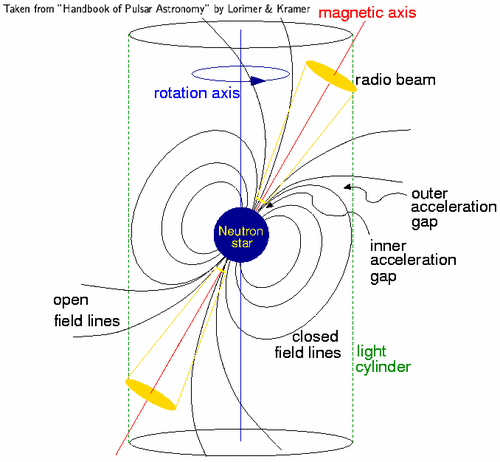
\includegraphics[width=0.7\textwidth]{figures/lhmodel.png}
\caption{Shows conventional model of rotating neutron star (lighthouse model). Image obtain from \citep{handbook}.  }
\label{lhmodel}
\end{figure}
\end{center}   
        \begin{figure}[h] \centering
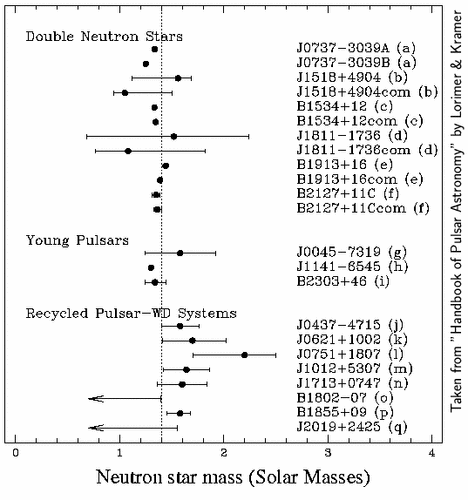
\includegraphics[width=0.6\textwidth]{figures/Mass.png}
\caption{The plot of pulsar with known mass with median value around 1.3 $M_\odot$ agree well with the canonical mass. Image from \cite{handbook} which is adapted from \citep{stairs2004pulsars}}
\label{mass}
\end{figure}

    \paragraph{} Due to angular momentum conservation, when the core of the progenitor star collapses into a neutron star.  The rotation period of the NS must increase. After that, the spin period will increase with time due to energy loss through magnetic dipole radiation process. Giving the rotational energy to be 
    \begin{equation}
    E=\frac{1}{2} I \Omega^2.
    \end{equation}
    the energy loss ($\dot{E}$) describe by 
    \begin{equation}
    \dot{E}=-I\Omega\dot{\Omega}\simeq 3.95\times10^{31}erg s^{-1} (\frac{\dot{P}}{10^{-15}})(\frac{P}{s})^{-3}.
    \end{equation}
    Where \textit{I} is the moment of inertia. $\Omega$ represents the angular velocity. Assume that pulsars are similar to spinning magnetic dipoles. The energy loss from  a pulsar with mass \textit{m} and misalignment between magnetic pole to rotation pole $\alpha$ is 
   
   \begin{equation} \label{Edotdipole}
   \dot{E}_{dipole}=\frac{2}{3c^3}|m|^2\Omega^4 \sin{\alpha}^2
   \end{equation}
   Assume that all of the energy loss from pulsar is magnetic dipole radiation gives us 
   \begin{eqnarray} 
   \dot{E}_{dipole}=\dot{E}\\
   \frac{2}{3c^3}|m|^2\Omega^4 \sin{\alpha}^2=-I\Omega\dot{\Omega}
   \end{eqnarray}
   Then the relation between $\dot{\Omega}$ and $\Omega$ is
   \begin{equation} \label{omegadot}
   \dot{\Omega}=\frac{2|m|^2\sin{\alpha}^2}{3Ic^3}\Omega^3.
   \end{equation}
   to simplify the solution, equation \ref{omegadot} can be written as $\dot{\Omega}=K\Omega^3$. Using $\Omega=2\pi \nu$.
   \begin{equation} \label{f}
   \dot{\nu}=-K\nu^{n_i}
   \end{equation}
 A breaking index ($n_i$) is 3 for dipole dominated case. However, the other sources of energy loss might also effect in this process. Measuring breaking index (n) allow us to test the energy loss mechanism from only $\nu$ and $\dot{\nu}$. By differentiating Equation \ref{f}.
   \begin{equation} \label{index}
   n_i=\frac{\nu \ddot{\nu}}{\dot{\nu}^2}
   \end{equation}
    $\nu$,$\dot{\nu}$ and $\ddot{\nu}$ are measurable only in limited conditions. Moreover,  measuring  $\ddot{\nu}$ is possible only with young pulsar with a large $\dot{\nu}$.  As a result,  on a small number of pulsars that can measure the spectral index. The result from the observation of spectral index  lying between $0.9 \leq n \leq  3.2$ ( \cite{Hamil:2015hqa} and \cite{Archibald:2016hxz}). Wide range of breaking index indicates that pulsars energy loss are not dominated by only magnetic dipole radiation. Moreover, an integral of Equation \ref{f} combined with the fact that $\Omega=\frac{2\pi}{P}$, giving that the approximate time from the pulsar at period $P_0$ to decrease to any given P for constant $\dot{P}$ is
    \begin{equation} \label{T}
   T=\frac{P}{(n-1)\dot{P}}[1-\frac{P_0}{P}^{n-1}]
   \end{equation}
   If we assume that the energy loss is purely magnetic dipole (n=3) and $\frac{P_0}{P}<<1$. Equation \ref{T} can be written as  
   
   \begin{equation} \label{tc}
   \tau_c \equiv \frac{P}{2\dot{P}} \simeq 15.8 Myr (\frac{P}{s})(\frac{\dot{P}}{10^{-15}})
   \end{equation}
 $\tau_c$ is defined as characteristic age which gives us an approximate age of a pulsar. Again, assuming magnetic dipole case. The surface magnetic field is  
    \begin{equation}\label{B}
    B_{surf}=\sqrt[2]{\frac{3c^3IP\dot{P}}{8\pi^2R^6sin \alpha^2}},
    \end{equation}
    Using canonical properties of pulsar with $\alpha$=90. Equation \ref{B} can be arranged as
    \begin{equation}
    B_{surf}=3.2x10^{19}\sqrt[2]{P\dot{P}}
    \end{equation}
 From this equation, the magnetic field of a pulsar can be approximated simply with only P and $\dot{P}$. From current pulsar population, $B_{surf}$ range from $10^{11}-10^{13}$ G. These values agree well with measurement from X-ray spectra \citep{coburn2002magnetic}, \citep{bignami2003magnetic}, and \citep{kouveliotou1998x}.  
    
\paragraph{} ~\cite{conway1962radio} shown that a discrete radio source (later found to be a pulsar) have spectral that follows power laws index as $S_{mean} = f^a_{obs}$ while $S_{mean}$ is means flux density, f is observing frequency and a is a spectral index with mean value of -1.8 ~\citep{maron2000pulsar}. This minus spectral index indicates that pulsars are brighter in low frequency observation.      
   
\section{Pulsar population} \label{pulsartype}
    \paragraph{} The previous section shows that characteristic age $\tau_c$ and surface magnetic field $B_{surf}$  can be described only with P and $\dot{P}$ in dipole dominated case. As a result, one of the most useful tools to study pulsars populations is  ``P- $\dot{P}$'' diagram as Figure ~\ref{ppdot}.  The diagram shows us five different types of pulsars, young pulsars, magnetars, ordinary pulsars, mildly recycled pulsars and recycled pulsars. 
    
        \begin{figure}[h] \centering 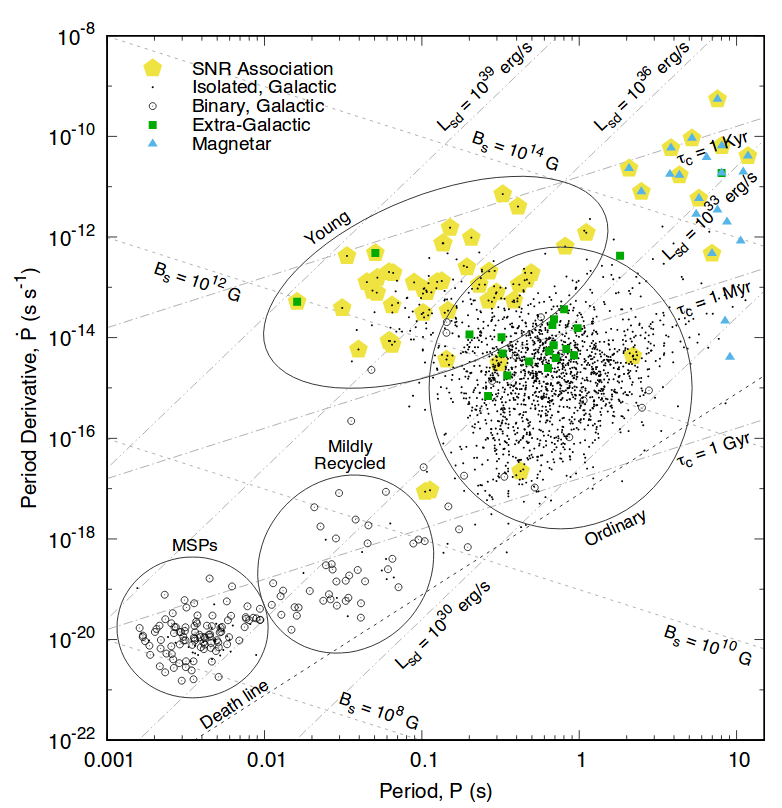
\includegraphics[width=0.7\textwidth]{figures/P-pdot.png}
\caption{ $P- \dot{P}$ diagram which shows five kinds of pulsar young pulsar, magnetar,  ordinary pulsar, mildly recycled pulsar and millisecond pulsar. Quantities such as $B_{surf}$, $\tau_c$, and $L_{sd}$ are calculated using purely magnetic dipole radiation model.  The death line describes the theoretical region where pulsar's magnetic field can not make radio emission. Image from ~\cite{Alex}}
\label{ppdot}
\end{figure}

\subsection{Young and Ordinary pulsars}
%%\paragraph{} talk briefly about definition, evolution, missing population as well as SNR timescale.

\paragraph{} The definition of young pulsars are pulsars at $\tau_c < 100000$ years. These pulsars are mostly associated with SNR. Young pulsars have relatively wide range of period from 0.01 s to 1s and $\dot{P}$ greater than $10^{-15}$. Due to high $\dot{P}$, this type of pulsars are possible to measure $\ddot{P}$ and $\nu=\frac{1}{P}$ which is important for understanding the radiation process. Young pulsars occasionally \textit{glitch} which means rapidly changed in $P$ and $\dot{P}$. \cite{link1992pulsar} proposed that glitches are an effect of angular momentum transfer inside the pulsar. Glitches can be used as a probe for pulsar moment of inertia. After a few hundred years, young, energetic pulsars lose their energy and eventually move to the lower left in Figure ~\ref{ppdot} to the largest population in the diagram, ordinary pulsars. Ordinary pulsars have $\tau_c$ range between $10^5 - 10^9$ years. The period is approximately 0.1 to a few seconds. Ordinary pulsars without mass transfer from its companion will lose their energy and ended up in  ``death line" ~\citep{chen1993pulsar}. However, not all of the pulsars are radiate purely magnetic dipole radiation. As a result, some pulsars might be detectable beyond the death line.  An example of this type of pulsar is PSR J2144-3933 that has a spin period of 8.51s. Detection of pulsar beyond death line indicates possibility of different radiation process ~\citep{zhang2000radio}.        


\subsection{Magnetars} \label{magnetar}

\paragraph{} Magnetars are a group of pulsars located in the top right part of the ``$P-\dot{P}$" diagram. Magnetars are highly associated with gamma ray bursts powered by their magnetic field ~\citep{duncan1992formation}. Some magnetar might even emit electromagnetic waves that more energetic than $\dot{E}_{dipole}$ called anomalous X-ray pulsar which implies that magnetars might have difference radiation process. Magnetars spin period are between $\sim$ 2 to 12s with high spin down ($10^{-15}-10^{-9}$). High spin down implies that this type of object has a high $B_{surf}$. This is the reason why this type of object called ``magnetar''. Slow period and high spin down imply the short life before it enters the death line in $P-\dot{P}$ diagram.  Moreover, some magnetars are not observable in radio frequency as know as radio quiet  magnetars. To date, there are only 29 magnetars discovered so far ~\citep{Olausen:2013bpa}.


\subsection{Mildly recycled and Recycled pulsars}

\begin{figure}[h] \centering 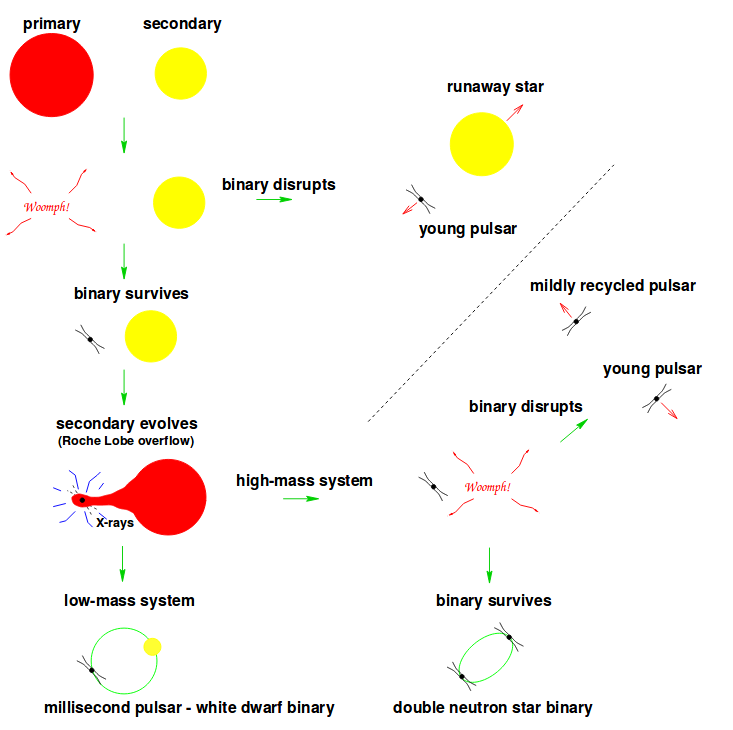
\includegraphics[width=0.75\textwidth]{figures/evo.png}
\caption{Theory of pulsar evolution in the binary system throughout their lifetime. For a binary system with high mass star, after the higher mass star ends its life, passing the supernova process. If the companion could not survive this process, it will be dispatched with large proper motion. However, this system still can evolve if this system can survive this process until the companion star ends its life. For low mass companion star case, the nova at the end of its life is not energetic enough to destroy the system. The result from this process is circular orbit system between NS and WD. For high mass companion case, the supernova at the end of its life is enough to change the orbit eccentricity. If the system can survive, the result of this process is a highly eccentric system of double pulsars. However, if the system could not survive the supernova, the resulting system is high proper motion mildly recycled pulsar from the first pulsar and young pulsar from the companion.   }

\label{evo}
\end{figure}

\paragraph{} Ordinary pulsars interacts with companion stars through mass transfer.  The angular momentum transfer is making them spin faster. As seen in Figure ~\ref{ppdot}, ``faster" pulsars like recycled pulsars and mildly recycled pulsars are mostly associated with binary systems. This process will make pulsar move to the lower left side of $P-\dot{P}$ diagram while losing their surface magnetic field by electromagnetic radiation. Resulting in relatively fast pulsar with a period between 0.01-0.2 s but with low $\dot{P} ~\sim 10^{-18}$. This type of pulsar known as recycled pulsars. In this thesis, I will refer pulsar that spins faster than 20 ms as millisecond pulsar. Recycled pulsars also have the smallest spin down because these pulsars have low-surface magnetic fields making their periods highly stable. Stable period characteristic of recycled pulsars could introduce some application for precise time measurement.  

 \section{How do pulsar signals propagate ?}
 \paragraph{} After pulsars emitted a signal, the signal emitted from a pulsar will travel throughout the interstellar medium (ISM), introducing some propagation effects. Two major effects are dispersion and scattering which will be discussed in this section.   
    \subsection{Pulse dispersion} \label{Pulse_dispersion}
\paragraph{} Travelling throughout the Galaxy, the emission from pulsars experienced different wave group velocity depends on frequencies. Refractive index which describes the velocity of electromagnetic waves in different mediums are described as equation ~\ref{rindex}, 
\begin{equation}\label{rindex}
\mu=\sqrt{(1-\dfrac{\nu_p}{f})}=\dfrac{v_g}{c}.
\end{equation} 
Where $f$ is the wave frequency, $\nu_p$ is plasma frequency, $v_g$ is group velocity and $c$ is a speed of light. Plasma frequency $\nu_p$ can be written as equation ~\ref{fp},
 \begin{equation}\label{fp}
 \nu_p=\sqrt{\dfrac{e^2n_e}{\pi m_e}},
  \end{equation} 
$n_e$, $e$ and $m_e$ are electron density, charge, and electron mass respectively. The light travel time along length L can be calculated from an integral of  
\begin{equation}\label{lighttraveltime}
 t=\int_{0}^{L}\dfrac{dl}{v_g}=\dfrac{L}{c}+\dfrac{e^2 \int_{0}^{L} n_e dl}{2\pi m_e c f^2}.
\end{equation} 
The first term describes light travel time in vacuum, while the second term describes delay caused by frequency dependent refractive index. To simplify the equation, the dispersion measure ($DM$) is defined as  
\begin{equation}
\label{DMdef}
DM=\int_{0}^{L} n_e dl,
\end{equation}
The time delay part from Equation \ref{lighttraveltime} can be re-written as    
\begin{equation}
\label{delaytime}
t=\dfrac{e^2}{2 \pi m_e c }\dfrac{DM}{f^2}=4.15\cdot 10^6 \dfrac{DM}{f^2}\,s.
\end{equation}
The DM is expressed in $cm^{-3} \, pc$ and $f$ is in MHz. The effect from time delay is observable only if the radiation is not continuous. From Equation ~\ref{delaytime}, the DM is estimated from 
\begin{equation}
\label{DMcal}
DM=\dfrac{\Delta t}{4.150\cdot 10^6}(f_{ref}^{-2}-f_{chan}^{-2}).
\end{equation}
  $\Delta t$ is difference of time delay between reference frequency ($f_{ref}$) and channel frequency ($f_{chan}$). The example of this effect on pulsar is shown in Figure \ref{DMplot}. Moreover, Equation ~\ref{delaytime} shown that this effect would be small for high frequency observation. This effect will smear out the signal causing difficulty for detecting pulsar in high DM region. The way to correct for this effect will be discussed in Section \ref{DDM}.    
\begin{figure}[h] \centering
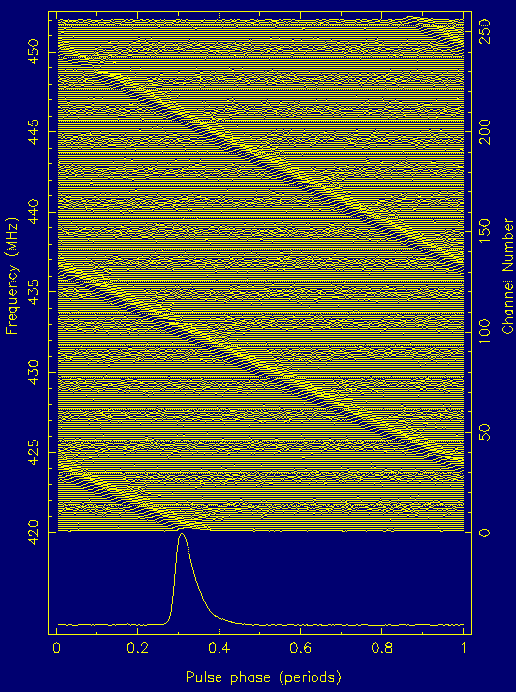
\includegraphics[width=0.5\textwidth]{figures/disp.png}
\caption{Shows effect of dispersion on a pulse of a pulsar. This effect makes lower frequency arrive later than high frequency. Image obtain from http://www.jb.man.ac.uk/distance/frontiers/pulsars/section4.html.  }
\label{DMplot}
\end{figure}
   \paragraph{} The DM represents the number density of electron along the line of sight to the source as Equation ~\ref{delaytime}. The simplest way to describe an electron density distribution in the space is to imagine it to uniformly distributed. The typical value for $n_e$ in our Galaxy is 0.03 $cm^{-3}$ \citep{ables1976hydrogen}. However, our Galaxy is much more complicated than the uniform distribution. By taking account of the shape of the Galaxy and carefully measuring the distance from many pulsars to the Earth. The model of free electron distribution can be describes ~\citep{cordes2003ne2001} and ~\citep{yao2017new} as shown in Figure \ref{nedist}.  As a result, the electrons distribution can be used to estimate the distance to the source if we know the density distribution. On the other hand, if the distance to pulsars is measured by other methods, the electron density can be evaluated. 
   
   %As a result, DM can be used as a probe to measure the distribution of free electrons in the universe as well as the distance between a pulsar to the Earth.     
\begin{figure}[h]
\centering
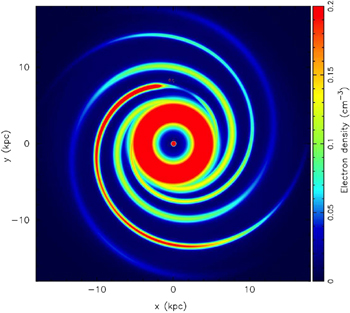
\includegraphics[width=0.5\textwidth]{figures/nedist.jpg}
\caption{Simulated electrons density distribution in the Milky Way galaxy show the complicated structure of our galaxy from the YMW16 model. Image obtained from \citep{yao2017new}  }
\label{nedist}
\end{figure}

    
    \subsection{Pulse scattering}
\paragraph{} When coherent electromagnetic waves from pulsars propagate through ISM, this cloud of ISM changes the signal's path length which makes an offset in the pulse phase creates diffraction pattern and phase delay as Figure ~\ref{scatt}. The result is a broader pulse profile with an exponential decay tail. This effect is called a scattering. 

 \begin{figure}[h] \centering 
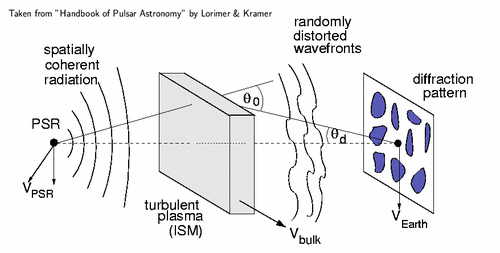
\includegraphics[width=0.8\textwidth]{figures/scatt.png}
\caption{A coherence signal from pulsar being perturbed by ISM causing an incoherence phase or pulse broadening. Image obtain from \citep{handbook}  }

\label{scatt}
\end{figure}

The exponential decay is defined as $I=I_0 e^{\frac{t}{\tau_s}}$ where $\tau_s$ defined as scattering time. $\tau_s$ can be measured by deconvolution of pulse profile with an exponential decay function. For thin screen case, it predicts that $\tau_s \propto f^{-4}$ \citep{xu2017scatter}. In this case, a pulse from the pulsar is expected to be larger in low frequency which reduce high of the peak as shown in Figure \ref{pscatt}. As a result, this effect can be reduced by observing at the higher frequency.

    \begin{figure}[h] \centering 
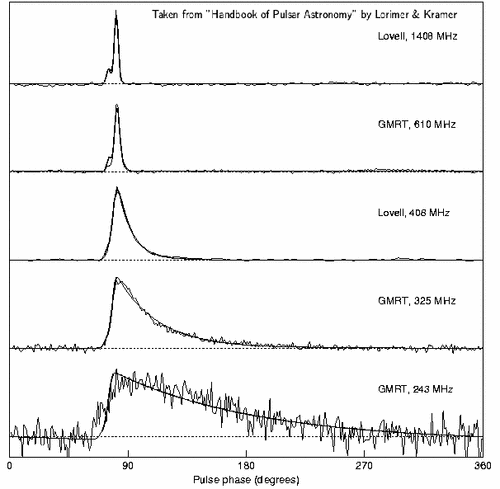
\includegraphics[width=0.5\textwidth]{figures/pulsescat.png}
\caption{Pulse profile from the same pulsar but observed with difference frequency shows the exponential decay tail. The effect is increased for low frequency observation making pulsar harder to detect. \citep{handbook}  }
\label{pscatt}
\end{figure}

\paragraph{} Since both dispersion and scattering are originate from the ISM, they are expected to be correlated. This correlation is shown by ~\cite{Bhat:2004xt}. The correlation between DM and $\tau_s$ being shown on Figure ~\ref{t_dm}. Consequently, Pulsars in a high DM environment such as at the centre of the Galaxy are expected to have boarder pulse.  

    \begin{figure}[h] \centering
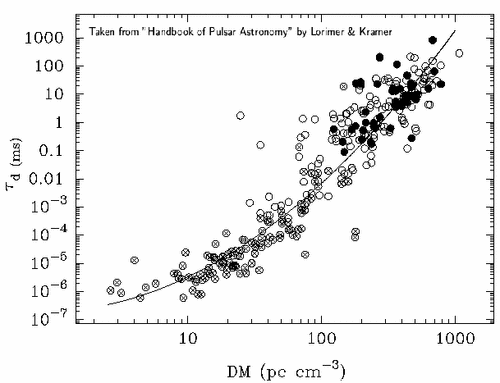
\includegraphics[width=0.5\textwidth]{figures/t_dm.png}
\caption{Show a correlation between DM and $\tau_s$. Image from \citep{handbook}  }
\label{t_dm}
\end{figure}

\section{Pulsars as physics tools}
    \paragraph{} Pulsars can be used as tools for study many aspects of physics, e.g. an array of pulsars can be used as a tool for detection of nano-hertz gravitational wave ~\citep{doi:10.1093/mnras/stw347}. Following subsections will demonstrate some way to use pulsar as physics tools.  

    \subsection{Stellar and Pulsar population} 
    \paragraph{} The current pulsar population is biased due to selection effect from the observation sensitivity making pulsars located far away from the earth or weak pulsar are harder to detect as Figure ~\ref{pdist}. As a result, finding more pulsar as many as we could help us the get a better understanding in our theory of pulsars formation and their progenitor stars. The better understanding of the theory of pulsar formation leads to many application such as predict rate of NSs merging. NSs merging event estimation is essential for understanding for the creation of heavy elements like the gold in our galaxy ~\citep{Thielemann:2017acv} and expected number observable gravitational waves ~\citep{0034-4885-72-7-076901}.
        \begin{figure}[h] \centering
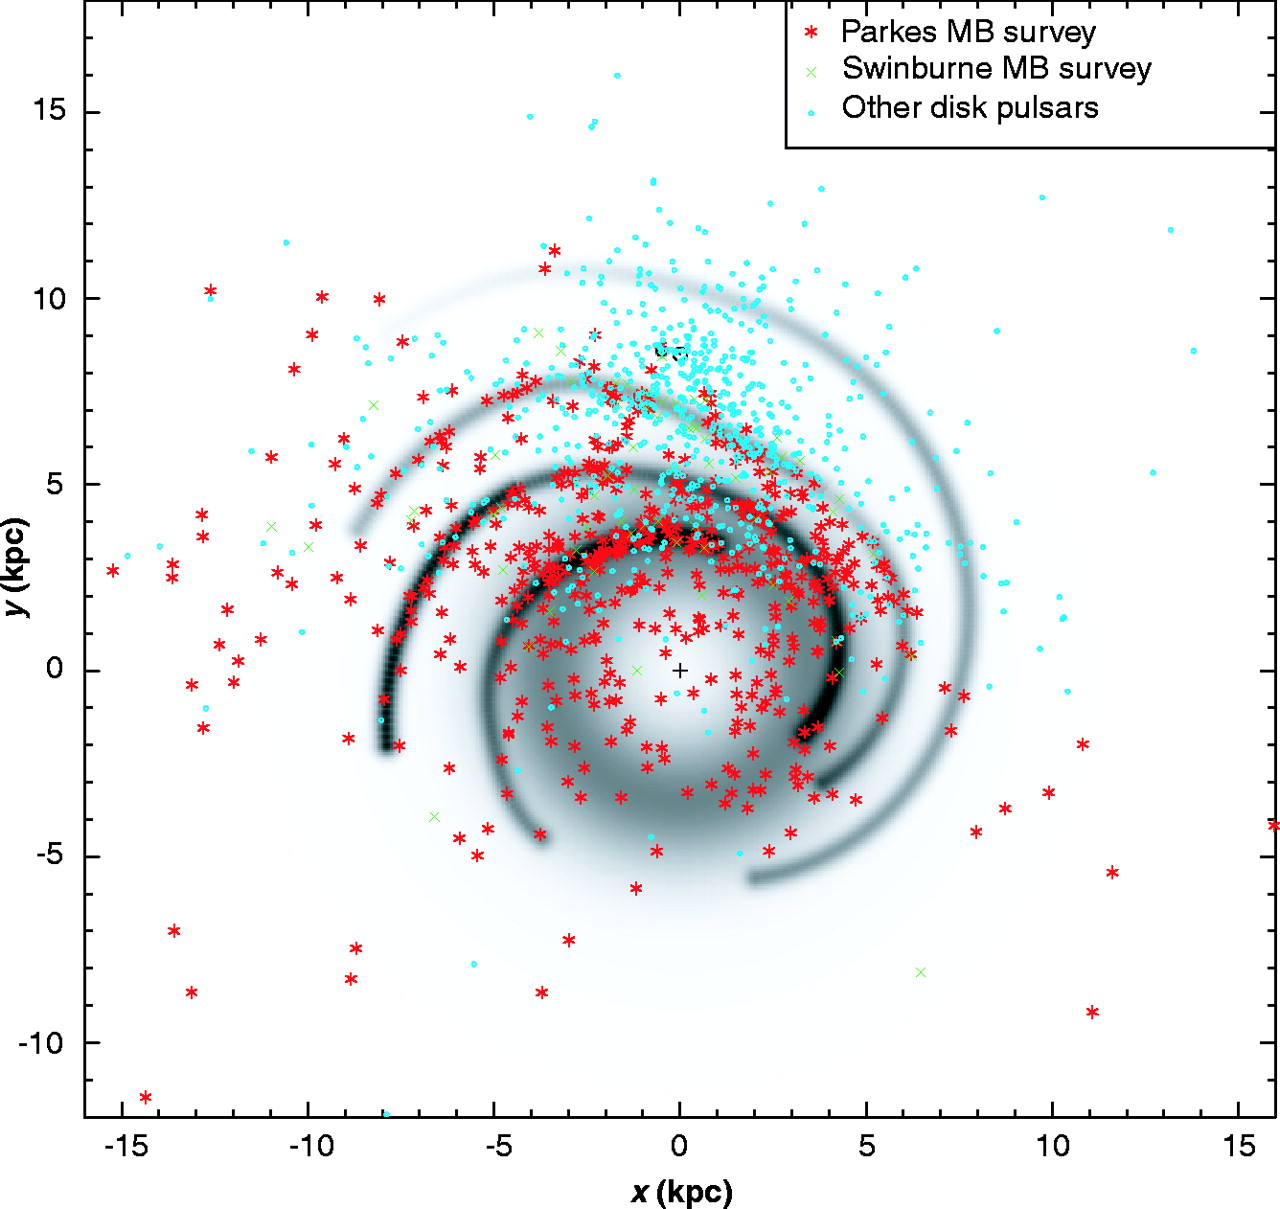
\includegraphics[width=0.4\textwidth]{figures/F1_large.jpg}
\caption{The distribution of pulsar in our galaxy shown underlying population missing due to observation sensitivity . Image from \citep{Manchester542}  }
\label{pdist}
\end{figure}
    \subsection{ISM distribution in the Galaxy}
    \paragraph{} As mentioned in Section \ref{Pulse_dispersion}, studying pulsars gives us information about our Galaxy ISM distribution. Moreover, pulsars are born in supernova explosions which kick pulsars out of the Galactic plane made them well distributed in all direction from the Earth. Widely distributed properties can be used to study our Galaxy in 3D which is not allows in the other objects because they are typically located i the galactic plane.  As a result, pulsars can be an effective probe for the Galactic electron distribution. This could lead to the model of our galaxy's free electron distribution. Moreover, pulsar can be used to study large-scale structure of Galaxy magnetic field by studying the relation between DM and effect from Faraday rotation~\citep{doi:10.1111/j.1365-2966.2008.13188.x}. 
    
    \subsection{Physics in extreme gravitational field}
    \paragraph{} Pulsar are dense objects which have a strong gravitational fields that are impossible to create on the Earth. As a result, pulsars can be used to test general relativity and modified gravity theories. For example, a double neutron star system PSR B1913+16 give the first detection of gravitational wave radiation as GR predicted that the orbit will change in the order of a centimetre per day ~\citep{weisberg2004relativistic}. Moreover, the double pulsar system is used to test five separated GR predictions with uncertainties of $\sim$ 0.05  \%  ~\citep{kramer2006tests}.  
    \paragraph{} Not only double pulsar systems but also other types of pulsar-binary can be used as physics tools. For example, NS-WD binaries are used as tools for testing the strong equivalence principle ~\citep{zhu2018tests} as well as the universality of free falling ~\citep{PhysRevLett.120.241104}. An NS-BH binary system which still not discovered will also be an excellent tool for strong equivalence principle in a stronger field than NS-WD system. 
        
  % \paragraph{} The Event-Horizon-Telescope Collaboration (EHTC) is aiming to image a shadow of the supermassive black hole at the centre of our galaxy (Sgr A*). However, ~\cite{mizuno2018current} suggest that only an image is not able to distinguish between the predicted result from GR and alternative theory. One of the suggestion is to find pulsar that orbiting around Sgr A* and combine that with an image.      
  
   \subsection{Physics of super-dense matter}
    \paragraph{} Due to the dense property of pulsar which it is not possible to produce on the Earth, binary pulsars are one of the best tools for studying the dense matter. For example, each equation of state predicts different maximum and minimum pulsar mass and radius. Moreover, glitches can also be used as a tool for study moment of inertial of neutron stars ~\citep{link1992pulsar}. Equation of states can be ruled out ~\citep{ozel2016masses} by measuring the mass of pulsar in binary system period or Shapiro delay  

\section{Thesis outline}
    \paragraph{} Methods for pulsar searches will be introduced in chapter ~\ref{Methods}. This chapter will mainly talk about the different methods to find pulsars, advantages and disadvantages of each method. Also, I will talk about the method for binary pulsar search and how to get rid of radio interference (RFI). Method for de-dispersion will be included here.
    \paragraph{} Chapter ~\ref{RFI} will introduce a new method of RFI mitigation from pulsar candidates database. This method is aiming to speedup pulsars candidate selection by investigating fake candidate that originate from the earth. 
    \paragraph{} Introduction various pulsar surveys will be discuss. Moreover, result of pulsar discovery and confirmation from Fast Folding Algorithm (FFA) pulsar search pipeline with acceleration search in various surveys will be discussed in Chapter ~\ref{FFA_c}. 
    \paragraph{} In chapter ~\ref{Con}, thesis conclusion and the plan will be introduced.
    
\chapter{Methods for pulsar searching} \label{Methods}
\paragraph{} After signals from pulsar pass throughout the ISM and arrive the radio telescope, the telescope's system will convert this analogue signals to digital signals ready to be processed. In order to detect weak pulses/pulse from a pulsar, three different techniques have been used. In this chapter, I will talk about The fast Fourier transform (FFT), The fast folding algorithm (FFA), and single pulse search. However, if this pulsar is in binary or more complicated system, signals from this pulsar will suffer from Doppler's shift.  Method to prepare the data and get rid of radio frequency interference (RFI) and dispersion will also be discussed here. 
    \section{Data acquisition}
		%\paragraph{} Dish collects the radiation from the source. Amplified and down convert by fronted. Convert from AC/DC by backed.  
		\paragraph{} After the signal arrives the telescope, the dish will focus the signal into the primary focal plane. As the signal from a pulsar is typically weak, the collaging area needs to be large. Examples of telescope that is used for pulsar observation are The 64-m Parkes radio telescope in Australia, the 100-m Green Bank telescope in the US, the 300-m Arecibo telescope in Puerto Rico, and 100-m Effelsberg telescope. Different dish size can affect the angular resolution by 
        \begin{equation} \label{angular_res}
        \Theta \approx \frac{c}{D \times f_{obs}}.
        \end{equation}
        When c is the speed of light, D is the diameter and $f_{obs}$ is observing frequency. Note that, this equation can be used only in far field case.
        \paragraph{} At the focal plane, the receiver will amplify the signal as soon as possible. Then, the bandpass filter will filter only selected band of radio frequency (RF). In order to reduce signal loss, the mixer attached with a local oscillator (LO) will down convert the RF to lower intermediate frequency. This part called Fronted. 
		\paragraph{} Backed is where the data get digitised from analogue to digital data. Digitized data will be analysed depends on the observation backed. In this work, only the pulsar search backed will be mentioned. In pulsar search backed, the digitised data will be streamed to Field Programmable Gate Array (FPGA) which will perform polyphase filterbank fast Fourier transforms (see more in Section ~\ref{FFT}) to channelise the signal into many individual narrow frequency channels. This data will be stored with the two polarisations summed and be ready to be  proceed.  
            \section{Data preparations} 
            \paragraph{} After the data is passing throughout backed system. The data will be processed in order to get the weak signal from the pulsar. First, we need to get rid of the radio frequency interference (RFI). Moreover, we need to remove the effect from interstellar medium as before mentioned in  ~\ref{Pulse_dispersion}.    
            
   \subsection{RFI mitigation} \label{RFI_mit}
        \paragraph{} RFI created can decrease the detectability of the pulsar. The strong RFI can reduce the sensitivity of the instrument by decreasing the dynamical range and can create many artificial pulsar candidates in pulsar search pipeline. So, one of the first step of the pulsar search pipeline is to detect and remove a strong RFI. 
        There are many approaches of RFI removal techniques. The simplest way is to search for a strong signal in time and frequency domain and filtered it out. However, this method might confuse a bright transient or a bright pulsar with a bright RFI. Another way is using the fact that, RFI generated from the Earth will not suffer from dispersion and appeared as zero DM signal. As a result, this type of RFI is removed by filtered out the signal with zero DM. However, this method might affect the detectability of a pulsar with a long period because long period pulsar has a broad DM-curve (a relation between S/N and DM) as mentioned in ~\ref{DDM}. So, the pipeline might misunderstand that this pulsar is a RFI. ~\cite{Ng} suggested that disadvantages from these methods can be compromised by comparing candidate with other beams from the same observation. Since pulsars are located far from the earth and weak, so pulsars are likely to be detected in only one observation beam. On the other hand, RFIs are originated from the Earth and likely to be detected in every beam. As a result, by comparing zero-DM Fourier spectrum with all of the observation beams, we can get rid of periodic RFI.     
        
        \subsection{De-dispersion} \label{DDM}
%        \paragraph{} Effect of DM, De-dispersion in theory, Type, step 
       % \paragraph{} As mentioned before, an effect of ISM will make a signal in each frequency arrive the Earth at a different time. This effect is removed by introducing a delay in each frequency as Equation ~\ref{delaytime}.
       \paragraph{} There are two ways of performing de-dispersion. The simplest way is ``incoherent de-dispersion''. This method will divide the total bandwidth into several channels and applying proper time shift estimated from Equation ~\ref{delaytime} which is easy to apply and computationally inexpensive. However, this method is limited since each of the divided frequency band or ``sub-band'' retain some smearing. The alternative method is called ``coherent de-dispersion'' (~\citep{hankins1971microsecond} and ~\citep{hankins1975methods}) which is apply Fourier transformed (see more in Section ~\ref{FFT}) to the data and rotate the relative phase of each component Fourier spectrum by an amount that is proportional to the DM of the pulsar. Coherence de-dispersion is slower compared to the first method but be able to recover the original pulsar signal.      However, the DM for each pulsar is an unknown. As a result, the data need to be ``de-dispersion'' in a different DM. 
        \paragraph{} To optimise the calculation time for the search pipeline. The dispersion step size needs to be optimised as well. As we know that dispersion can reduce the S/N of the data by broadening the pulse profile. The apparent pulse width or effective pulse width for a top-hat pulse with an intrinsic pulse width of $W_{int}$ due to DM offset ($\Delta DM$) is 
        \begin{equation}
        W_{eff}=\sqrt[]{W_{int}^2+(8.3 \times 10^6 \times \frac{\Delta f}{f_c^3} \times |\Delta DM|)^2+t_{samp}}.
        \end{equation}
        When $\Delta f$ is the bandwidth of this observation. The reduce in S/N by an offset of DM is estimated by 
        \begin{equation}
        S/N \propto \sqrt[]{\frac{P-W_{eff}}{W_{eff}}}
        \end{equation}
        This relationship is shown in Figure ~\ref{DMcurve} and indicate that for long period or wide pulse width pulsar, the DM curve will be larger.       
                 \begin{figure}[h]
\centering
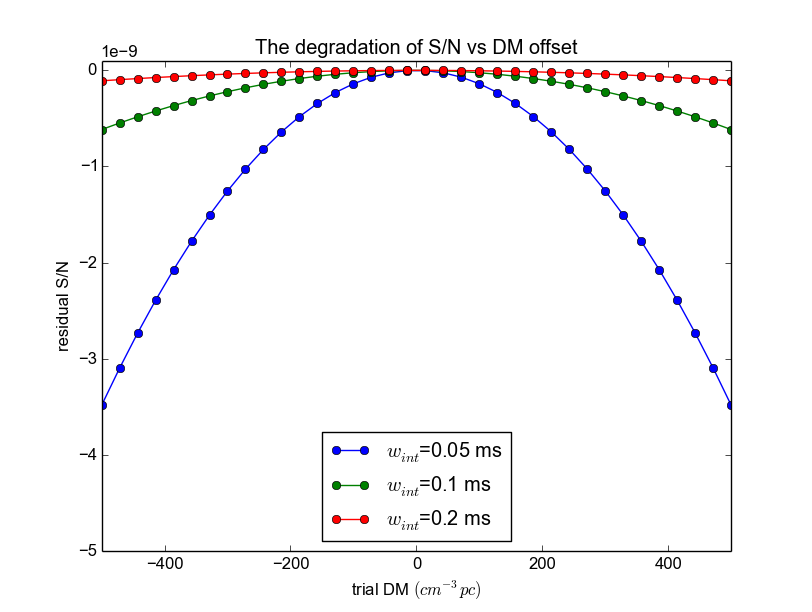
\includegraphics[width=0.80\textwidth]{figures/DMcurve-title.png}
\caption{Demonstration of Degradation of S/N by DM offset for  simulated 2s pulsar observed at $f_c= 430$ MHz and $\Delta f=$ 8 MHz.}
\label{DMcurve}
\end{figure}
        The dispersion step size can be calculated from giving the condition that if the dispersion time is smaller than sampling time, the S/N will be the same. The $i^{th}$ DM value is written by 
        \begin{equation} \label{dm_step}
        DM_i=1.205\times10^{-7} cm^{-3} pc (i-1)t_{samp}(f_c^3/\Delta f)
        \end{equation}        
        When $\Delta f$ is the total bandwidth in MHz. $f_c$ is the central frequency. At $i=n_{chan}+1$ or ``diagonal DM'', the dispersion delay across the bandwidth will be ``$n_{chan} \times t_{samp}$''. After the second diagonal DM is reached, the dispersion delay time on each channel becomes $2 t_{samp}$ which allows us to ``down sampling'' the data by the factor of two. This process can be repeated when the DM get higher to save the computational power. As a result, Equation ~\ref{dm_step} can be re-write as 
        
                \begin{equation} \label{dm_step_dig}
        DM_i=DM_{1}(i-1) Df 
        \end{equation}        
         
               When $DM_{1}$ is the first diaganal DM defined as $DM_1 = 1.205\times10^{-7} t_{samp}(f_c^3/\Delta f)$  and $Df$ is the downsampling factor. 

        
    \section{Algorithms for pulsar search}
    \paragraph{} After the data is de-dispersed. This data need to be "search" to see if there are any pulsar signal in that data. In this section, three of pulsar search method will be discussed.   
        	\subsection{Single pulse search (SP)} \label{SP}
        \paragraph{} The easiest way to search for a pulsar is to find any ``pulse'' that is strong enough in the time series. Imagine a time series with Gaussian noise. The ``pulse'' can be detected by searching for any signal that is stronger than certain standard deviation. In the best case where the pulse width is equal to sampling time ($t_{samp}$), ~\cite{cordes2003searches} shown that the S/N of the detected pulse is 
\begin{eqnarray}
S/N=\frac{S_{peak} W}{S_{sys}}\sqrt[]{\frac{n_p \Delta f}{W}}
\end{eqnarray}
Where $S_{sys}$ is the system-noise equivalent flux density, $n_p$ is the number of polarisations and $\Delta f$ bandwidth of the receiver, W is pulse width and $S_{peak}$ is the pulse amplitude. However, W is not always equal to $t_{samp}$ so, matched filtering algorithm needs to be applied to this time series. Matched filtering is down-sample the time series with different factor searching for the factor that gives the best S/N which is the factor where $W \approx t_{samp}$.

\paragraph{} Single pulse search allows us to detect the pulsar that emits a strong pulse like giant pulse emitter. Giant pulse emitter is the pulsar which can produce a pulse that more than ten times stronger than the mean pulse intensity. 
    	\subsection{The Fast Fourier Transform (FFT)} \label{FFT}
%        \paragraph{}Principle, equation, application to pulsar search, missing population 
        \paragraph{} Another way to search for pulsar is to search for any periodicity in the time series. The most successful technique for pulsar search is to take the Fourier to transform to the time series and study the Fourier frequency domain. However, since the time series is a discrete data which is not possible to apply Fourier transform directly. The discrete Fourier transform (DFT) is used instead for discrete times series ($\mathcal{T}$) with N data point. The $k^{th}$ Fourier component of DFT can be evaluated from        
 \begin{equation}
 \mathcal{F}_k=\sum_{j=1}^{N-1} \mathcal{T}_j exp(-2\pi ijk/N)
 \end{equation}
 where k is the Fourier frequency and $i = \sqrt[]{-1}$. From Nyquist sampling theory, the range of frequency spectrum that can obtain from DFT is $\frac{1}{t_{int}}<\nu<\frac{1}{2 t_{samp}}$ ~\citep{ransom2002fourier}. However, DFT is relatively slow because it requires $N^2$ floating point operation. The faster version of DFT is the fast Fourier transform (FFT) that require $Nlog_2(N)$ operation. Imagine the time series with $10^6$ samples, DFT needs $10^{12}$ operations while FFT takes only $6log_2 10$ hich is $\approx 10^7$ which is $10^5$ times faster. The improvement of FFT came from the properties of Fourier transform that $\mathcal{F}_{N-k}=(\mathcal{F}_k)*$ which makes DFT is symmetrical around $k=N/2$ which can reduce the number of operation ~\citep{FFT}. A Fourier spectrum $\mathcal{P}_j$ can be created from the summation between the real and imaginary parts of the Fourier components ($\mathcal{P}_k=|\mathcal{F}_k^2|$). The Fourier spectrum could be used to investigate the periodicity in time series as demonstrate in ~\ref{FFT_im}.  
 
 \begin{figure}[h]
\centering
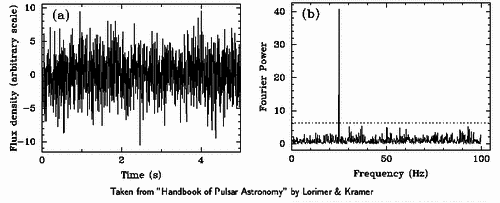
\includegraphics[width=0.80\textwidth]{figures/FFT}
\caption{Demonstration of applying FFT to a time series with a 25 Hz signal in the left side image. The result from the previous process is the power spectrum of this time series showing a peak at 25 Hz as shown in the right image. The dashed line in the right image showing the detection threshold. Images from ~\citep{handbook}}
\label{FFT_im}
\end{figure}
\paragraph{} Unfortunately, the pulsed signal that we are searching for have a pulse width which is a few percents of the period (0.2-25$\%$). This pulse width is also reference as ``duty circle'' $\delta$ which is the pulse width (W) divided by period (P), $\delta=W/P$. The time series with this narrow pulses will result in the Fourier frequency spectrum in fundamental frequency and many harmonics. A technique is known as ``incoherent harmonic summing'' was invented by ~\cite{taylor1969two} to maximise the detected S/N by adding lower harmonics to the fundamental spectrum as Figure ~\ref{FFT_ham}.

 \begin{figure}[h]
\centering
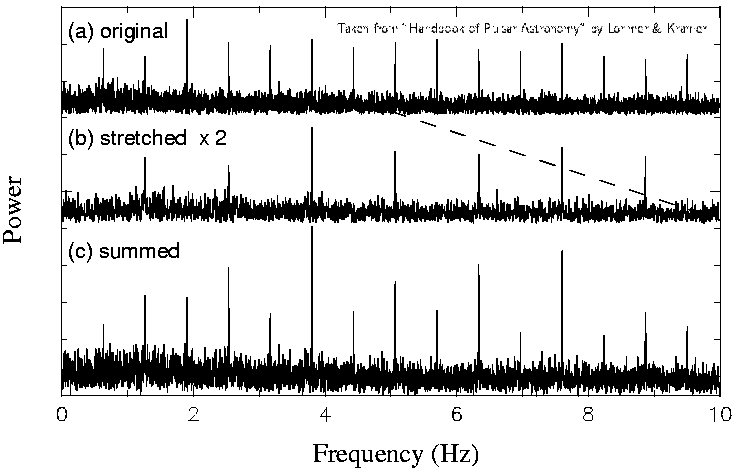
\includegraphics[width=0.8\textwidth]{figures/6_06.png}
\caption{Demonstration of applying harmonic summing by stretched other half of the spectrum by a factor of 2 and add that to the original spectrum. The process can increase the S/N by a factor of $\sqrt[]{2}$. Repeating of this process will increase S/N by large factor. Images from ~\citep{handbook}}
\label{FFT_ham}
\end{figure}
		%\paragraph{} To distinguish between real detection from random noise result, the significance of that signal needs to be determined. For a time series with Gaussian noise, ~\cite{handbook} shown that the minimum S/N of the signal that is real detection is 
        \paragraph{} For a time series with Gaussian noise, ~\cite{handbook} shown that the minimum S/N for significant detection is
        \begin{equation}
        S/N_{min}=\frac{\sqrt[]{ln[n_{trials}]}-\sqrt[]{\pi/4}}{1-\pi/4}.
        \end{equation}
		$n_{trials}$ is the total number of trial which is calculated from 
        \begin{equation} \label{n_trial}
        n_{trial}=N \times N_{dm} \times N_{acc}
        \end{equation}
        when $N_{dm}$  and $N_{acc}$is total number of trial DM and acceleration respectively. The probability limit of detecting random noise candidates is defined as ``False-alarm probability''  
\paragraph{} FFT is one of the most successful algorithm for pulsar search. However, FFT has limitation on long period pulsar (defined here as pulsar which has a period longer than 1 s) as shown in  ~\citep{kondratiev2009new}. The alternative search algorithm will be discussed in section ~\ref{FFA}.

        \subsection{The Fast Folding Algorithm (FFA)} \label{FFA}
       % \paragraph{} Principle, equation, application on pulsar search  
        \paragraph{} An alternative way to search for periodicity in any time series is to directly fold de-disperse time series with different period and searching for a pulse profile. However, brute-force folding algorithm needs $N[(N/n)-1]$ operations when n is the number of profile bin. This process is computationally expensive in a similar way with DFT. Shortly after an implementation of FFT in 1965 ~\citep{FFT}, ~\cite{staelin1969passive} implemented the fast-folding algorithm (FFA). FFA works by splitting a time series into a small fraction of n sample with the condition that $N/n$ is an integer power of 2 when N is the total sample number. The these dived time series will be combined in the different way which represents different period as ~\ref{FFA_im}. The folded profile p at $k^{th}$ bin is 
        \begin{equation}
        p_k=\sum_{j=0}^{N/P_0-1}\mathcal{T}_{k+jP_0}
        \end{equation}
        \paragraph{} FFA takes only $Nlog_2(N/n)$ operations. However, FFA still computationally expensive due to a high data sampling rate which makes FFA not possible to apply to large survey before. FFA shows many advantages in searching for a slow pulsar. For example, even the slow pulsar has a pulse width of $1\%$, this pulse with will be at least 10 ms (for 1 S pulsar). This means that the time series can be downsampling from $64 \mu s$ to $~\approx 1ms$ which makes N $\approx 156$ times smaller. This smaller N leads to less operation. Moreover, FFA gives a result in a fully coherent phase which can recover some sensitivity that lost in FFT ~\citep{kondratiev2009new}. The result from FFA by varying $N/P_0$ will be displayed in a periodogram that shows S/N for each trial period. The searching plan for FFA is written as 
        \begin{equation}
        P_{max}=P_{min}+\frac{P_{min}}{bins_{min}} \times n_{bins}
        \end{equation}
        When $bins_{min}$ is minimum searching profile bins. $n_{bins} $ is different between maximum and minimum profile bins. A demonstration of FFA search step is shown in Table ~\ref{FFA_step}. The sampling time for each period is selected from the fact that $t_{samp}$ for each period need to be at least $\frac{1}{bins_{min}}$. This can introduce huge downsampling factor $dfactor$. 
        
         \paragraph{} False alarm rate probability for FFA is directly related to profile significant. The probability of detection pulse profile with specific S/N by random Gaussian noise is written by 
                 \begin{equation}
        Prob(>S/N)=\frac{1}{n_{trial}}=\frac{1}{\sqrt[]{2\pi}} \int^{\infty}_{S/N} e^{-x^2/2}=\frac{1}{2} [1-erf(\frac{S/N}{\sqrt[]{2}})]
        \end{equation}
        the error function $erf(x)$ could be solved numerically. For more information see ~\cite{press1992numerical}. The number of trial in FFA is $n_{trial}=n_{FFA} \times N_{dm} \times N_{acc} $
         \begin{figure}[h]
\centering
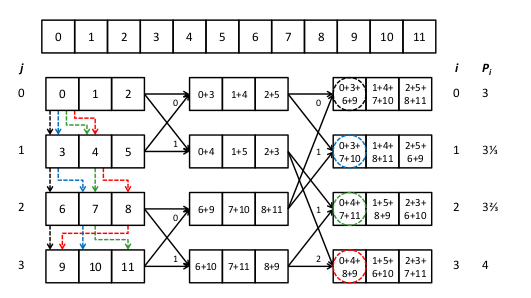
\includegraphics[width=0.80\textwidth]{figures/FFA.png}
\caption{Demonstration of applying FFA to a time series with N=12. The time series is folded into 4 different trial period. Each arrow represent the bin with same color circle. Image from  ~\citep{Andrew}}
\label{FFA_im}
\end{figure}
%		\paragraph{} The result from FFA by varying $N/P_0$ will be displayed in a periodogram that shows S/N for each trail period. 
        \subsection{Comparison between searching methods} \label{Com}
        \paragraph{} Investigating in each of search algorithm theoretical S/N is require in order to compare each of search method. First, single pulse search is basically search for signal that exceeds the noise with matching filter. The S/N for SP for a top hat pulse with flux S and width w is written as.   
		\begin{equation}
		S/N_{SP}=S_{peak} \cdot \sqrt[]{w} \label{snr_sp}
		\end{equation}       
        \paragraph{} FFT is more complicated because it applies harmonic summing to the data.~\cite{kondratiev2009new} shown that $S/N_{FFT}$ for H harmonic sum is  
        		\begin{eqnarray}
		S/N_{FFT}=\sqrt[]{\frac{\pi}{H(4-\pi)}} \sum^H_{n=1}[L^0_{1/2}(-N[S_{av}(1-\delta)sinc[\pi n (1-\delta)]]^2)-1] \label{snr_fft}
		\end{eqnarray}    
        When $L^0_{1/2}(x)$ is the generalized Laguerre polynomial $L^{\alpha}_{n}(x)$. $S_{av}$ is the average pulse flux which depends on pulse flux distribution. $\delta$ is the ``duty circle ($\delta$)'' defined by $\delta=w/P$
        \paragraph{} FFA is similar to SP but FFA is to detecting average pulse profile that integrate over number of pulses ($N_p$).  ~\cite{kondratiev2009new} proposed that S/N for FFA is  
        \begin{equation}
		S/N_{FFA}=S_{av} \cdot \sqrt[]{w} \cdot \sqrt[]{N_p}. \label{snr_ffa}
		\end{equation}
	\paragraph{} The comparison between FFA and FFT has been done by ~\cite{Andrew} and ~\cite{kondratiev2009new} as Figure . This comparison shows the advantage of FFA to FFT in searching for long period and narrow pulse width pulsar.  Diving Equation  ~\ref{snr_ffa} with Equation ~\ref{snr_sp} gives that 
    \begin{equation} \label{r}
    \frac{S/N_{FFA}}{S/N_{SP}}=\frac{S_{av} \sqrt[]{N_p}}{S_{peak}}
    \end{equation}
    
\begin{figure}[h] \centering
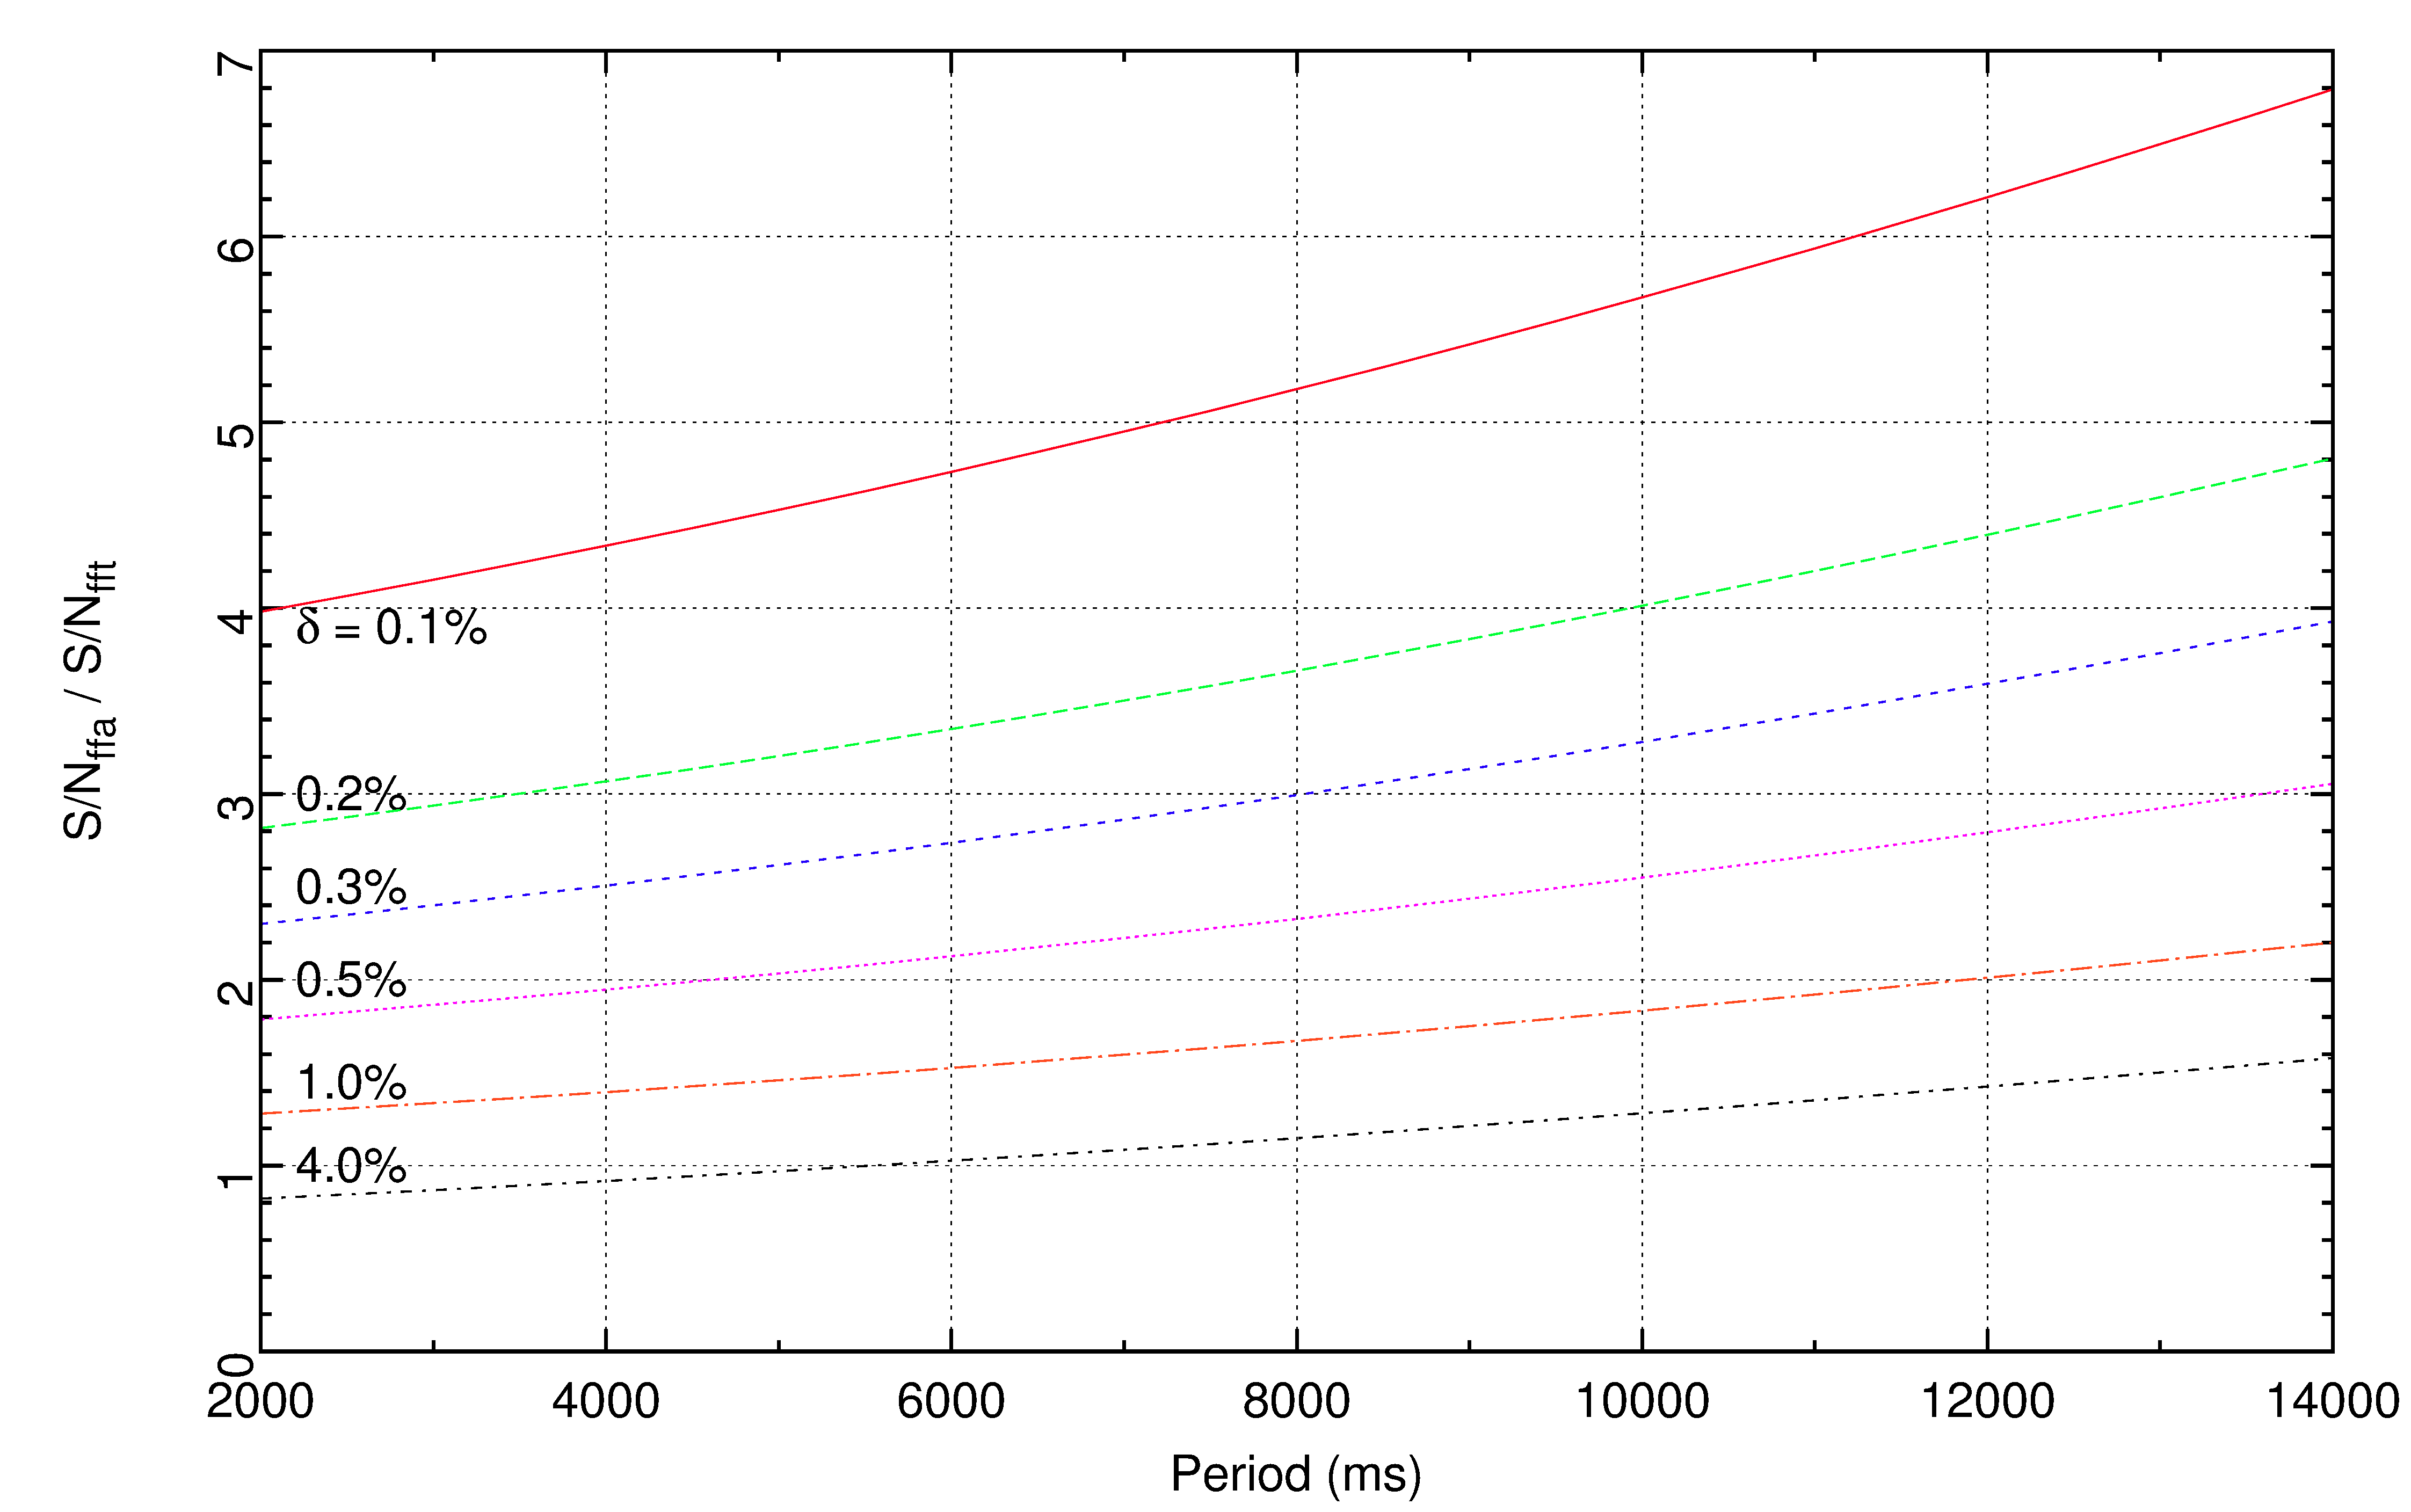
\includegraphics[width=0.80\textwidth]{figures/FFA_FFT.png}
\caption{The analytical prediction of the ration between $S/N_{FFA}$ to $S/N_{FFT}$ as a function of period and duty circle}
\label{FFA_FFT_com}
\end{figure}

	\paragraph{} ~\cite{keane2011transient} and ~\cite{mclaughlin2003searches} attempted to compare SP with other algorithms with ``lognornal'' pulse flux distribution which is typically observed from normal pulsar (\cite{cairns2001intrinsic}, \cite{johnston2001high}, and \cite{serylak2009simultaneous}) while pulsar that emits ``giant pulses'' which are pulses that more than 10 times stronger than average flux ~\citep{karuppusamy2010giant}. The pulse flux distribution for this type of pulsar are well describes by power laws. 
    \paragraph{} For lognormal distribution, the flux (S) distribution ($f(S)$) describes as 
    \begin{equation}
    f(s)=\frac{1}{\sigma \sqrt[]{2 \pi}} \frac{exp(-\frac{(ln S - \mu)^2}{2 \sigma^2})}{S}
    \end{equation}
    Moreover, the peak flux ($S_{peak}$) and average flux are 
    \begin{eqnarray}
     S_{peak}=exp(\sqrt[]{2} erfinv(1-\frac{2}{N})+\mu) \label{Speaklog}\\
    S_{av}=\frac{1}{2} exp(\mu+\frac{1}{2} \sigma^2) (1+erf(\frac{1}{\sigma \sqrt[]{2}} (ln S_{speak} - \mu)-\sigma^2)) \label{Savlog}
    \end{eqnarray}
   
   When erfinv(x) \footnote{see more https://docs.scipy.org/doc/scipy/reference/generated/scipy.special.erfinv.html} is inverse error function which can be solved numerically. ~\cite{cairns2001intrinsic} have evaluate $\mu 2.3$ and $\sigma = 0.096$ for Vela pulsar. \cite{weltevrede2006bright} also determined $\mu = 0.34$ and $\sigma = 0.99$ for lognormal model of PSR B0656+14. 
   
   \paragraph{} For Power-laws distribution, the distribution is given as 
\begin{equation}
f(S)=AS^{-\alpha} \label{fpower}
\end{equation}
    To make Equation ~\ref{fpower} converted, Pulses are assumed to emitted in a finite range between $S_1$ and $S_2$. The peak flux density is 
  \begin{equation}
  S_{peak}=\left\{
    \begin{array}{@{}ll@{}}
    [(\frac{N-1}{N})S_2^{1-\alpha}+\frac{S^{1-\alpha}_1}{N})]^{\frac{1}{1-\alpha}}, & \ \alpha \neq 1 \\ \\
    S_1(\frac{S_2}{S_1})^{\frac{N-1}{N}}, & \ \alpha = 1
  \end{array}\right. \label{Speakpo}
  \end{equation}
  the average flux is 
  \begin{equation}
  S_{av}=\left\{
    \begin{array}{@{}ll@{}}
    (\frac{\alpha-1}{\alpha-2})(\frac{x^{\alpha-2}-1}{x^{\alpha-1}-1}) S_{peak}, & \ \alpha \neq 1,2 \\ \\
    \frac{S_{peak}-S_1}{ln(S_{peak}/S_1)}, & \ \alpha = 1 \\ \\
    \frac{S_1 ln x}{S-S_1} S_{peak}, & \ \alpha = 2
  \end{array}\right.
  \end{equation}
   When $x = \frac{S_{peak}}{S_1}$ from re-written of Equation \ref{x} is 
   \begin{equation}
  x=\left\{
    \begin{array}{@{}ll@{}}
    [(\frac{N-1}{N})+\frac{1}{N}(\frac{S_2}{S_1})^{\alpha-1}]^{\frac{1}{1-\alpha}} (\frac{S_2}{S_1}), & \ \alpha \neq 1 \\ \\
    (\frac{S_2}{S_1})^{\frac{N-1}{N}}, & \ \alpha = 1
  \end{array}\right. \label{x}
  \end{equation}\paragraph{} The comparison between FFA and FFT is shown in ~\ref{FFA_SP_com}. This shows that,  normal pulsars are likely to be detected with FFA than SP search.  The condition that makes SP more effective that FFA is when the pulse period is longer than 2000 s which is way more longer than the longest period  pulsar.  For giant pulse emitter, ~\cite{keane2011transient} demonstrated that SP will be more effective for giant pulse emitter with flux distribution that follows power laws that $1<\alpha<3$.  The result from ~\ref{FFA_SP_com} agree well with this assumption.  
  
  \paragraph{} This means that FFA is useful in searching for a slow (P>1 s ) and wide pulse width pulsar while FFT is adequate for the fast spin pulsar. Moreover, SP is not useful for the ordinary pulsar in long integration time because as the integration time gets longer, the number of N also bigger increase $S/N_{FFA}$. SP become more effective when we are searching for giant pulse emitter pulsar as shown in Equation ~\ref{r}.  Giant pulse emitter an emitted pulse that is 1000 times brighter than average flux    ~\cite{karuppusamy2010giant}.  This means that the ratio between   $S_{av}$ and $S_{peak}$ is lower for this type of pulsar leading to more efficiency in SP. 


  \begin{figure}[h] \centering
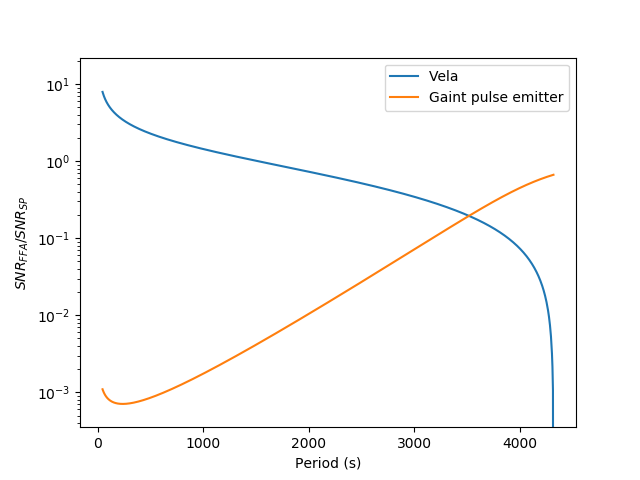
\includegraphics[width=0.80\textwidth]{figures/FFA-SP.png}
\caption{The analytical prediction of the ratio between $S/N_{FFA}$ to $S/N_{sp}$ as a function of period.  Gaint pulse emitter here is defined with a power law flux distribution of $\alpha$=3}
\label{FFA_SP_com}
\end{figure}
  
    \section{Binary pulsar search} \label{BS}
%	\paragraph{} Effect on binary motion to pulsar signal, time domain re sampling, acceleration search and 10 percent rule.   
	\paragraph{} Being in a binary system could change the apparent period of a pulsar. Changing of the period could make the emitting power to others spectrum/periodogram bins which can reduce the S/N ratio. One of the ways to recover this signal is the technique called ``time domain resampling''. Time domain resampling is resampled the time series into the rest frame of the pulsar. The core of this process begins with the relation between pulsar time interval $\tau_0$  as a moving emitter with velocity $V_1(t)$ and observer time interval $\tau$. 
\begin{equation}
\tau=\tau_0(1+V_1(t)/c)
\end{equation}
t is observed time, and c is the speed of light. If we assume that the acceleration ($a$) in along the observation time is constant ($V_1(t)=at_{obs}^2$), the equation above can be re-written as 
\begin{eqnarray}
\tau=\tau_0(1+\frac{at}{c})
\end{eqnarray} 
In this work, I will focus on applying acceleration search to FFA for the first time.

\paragraph{} We can search of pulsar with a constant acceleration by apply time domain resampling with different acceleration trails ($\delta a$). To calculate an optimal step size for acceleration trials for observation time $t_{int}$, the period in observer frame ($P$) need to change less than one pulse profile bin. The explanation of this method is similar to diagonal DM as explained in Section ~\ref{DDM}. The only situation where the signal can be loss from FFA is when the smearing time is more than a bin as Figure ~\ref{diag}.     In this work, we choose the pulse profile bin to be 1/128 of the trial period (P). ~\cite{Ralph} suggest that the different between $P$ and $P_0$ could even be $8 t_{samp}$. Moreover, we can see that the relation between $\tau$ and $\tau_0$ is quadric. As a result, the re-sampling time will be calculated from the middle of the observation ($t_{obs}/2$)to minimise this effect. The acceleration step can be calculated from
\begin{eqnarray}
8t_{samp}=\frac{\delta at^2}{2c}\\
a_0 = \frac{16c t_{samp}}{(t_{obs}/2)^2}\\
a_0 = \frac{64c t_{samp}}{2 t_{obs}^2}\\
a_i=a_0(i-1)Df \label{acc_step}
\end{eqnarray}
The testing result from this implementation could be found in Section ~\ref{AFFA}. From Equation ~\ref{acc_step}, we found that FFA has a potential for further optimisation by making acceleration step for each trial period. The ``constant acceleration assumption'' has to follow the condition that the observation time ($t_{obs}$) needs to be less than $10\%$ of the the orbital period $P_{orb}$ ~\citep{ransom2002fourier}.

\paragraph{} The acceleration range can be calculated from Kepler's third law with orbital inclination equal to $90^o$. The maximum acceleration magnitude is 
\begin{equation}
|a_{max}|=(\frac{2\pi}{P_{orb}})^{\frac{4}{3}}(T_\odot f)^{\frac{1}{3}}c
\end{equation}
where c is the speed of light and $T_\odot=GM_{odot}/c^3$. The mass function $f$ is 
\begin{equation}
f=\frac{m_c^3}{(m_p+m_c)^2},
\end{equation}
when $m_p$ is the mass of the pulsar assumed to be $1.4M_\odot$ and $m_c$ is the companion mass (see more at ~\cite{ng2015high}). 


\begin{figure}[h] \centering
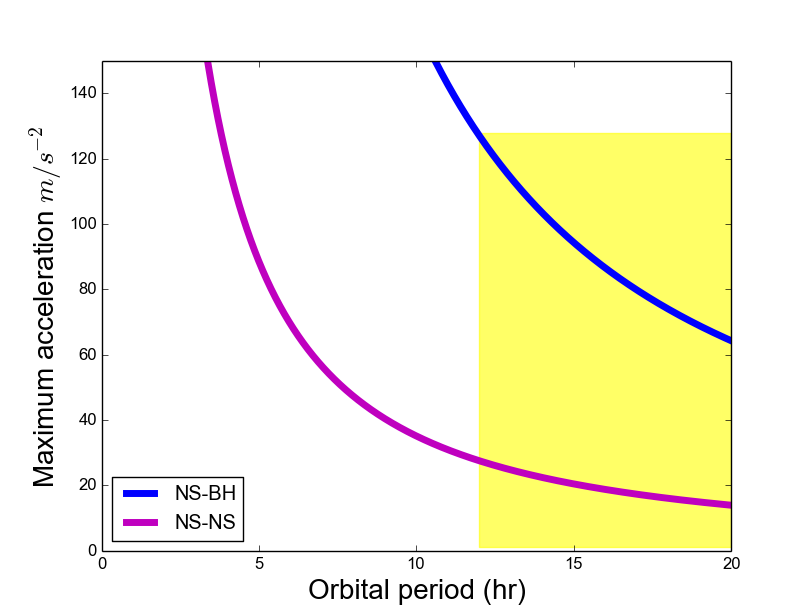
\includegraphics[width=1.0\textwidth]{figures/acc_plot.png}
\caption{Maximum acceleration for different orbital period ($P){obs}$) for pulsar with 37 and 1.4 $M_\odot$ companion. The yellow regions correspond to acceleration and orbital period where constant acceleration approximation is most effective to. }
\label{Fig:acc_range}
\end{figure}


    \section{Candidate selections}
   % \paragraph{} Whats difference between Pulsar and RFI ? 
    \paragraph{} After all the step above, the pulsar in the search range should be detected with significant S/N in multiple harmonics, DM, acceleration. So, the `candidate sifting' is required to identify if that candidate belongs to the same pulsar/RFI. The ``Sifting'' is grouping up all the harmonically related and find the best S/N candidate. All of the data will be plotted into many plots for each candidate called ``diagnosis plot''. Examples of RFI and pulsar candidates are shown in Figure ~\ref{J1745_p} and ~\ref{RFI_p} respectively. The first column from the left shows important numbers of this candidate. In the next column, shows the phase-time plot, integrated profile and the relation between S/N and pulse profile. The last column illustrates relations between S/N with DM, period and acceleration at that DM and Period. This ``diagnosis plot'' are modified by an FFA package called ``riptide'' with some modification of acceleration search. The detailed about ``riptide'' will be mention in Chapter ~\ref{FFA_c}
    \begin{figure}[h] \centering
    \subfigure[An example of a pulsar candidate. ]
    {
    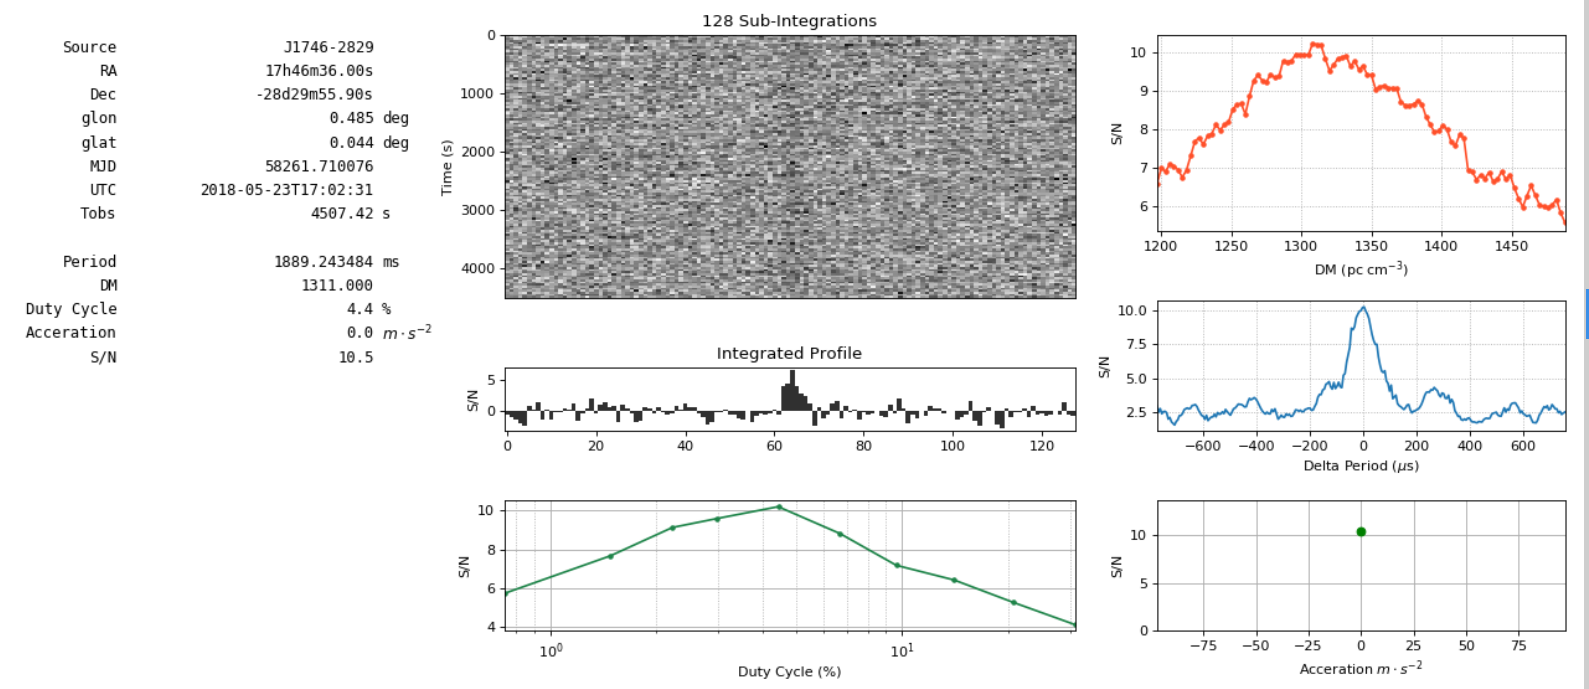
\includegraphics[width=1.0\textwidth]{figures/J1746-2829.png} 
    \label{J1745_p}
    }
	 \subfigure[An example of a strong periodic RFI showing low DM. Moreover, this candidate has a sinusoidal profile which is the signature of human-made RFI. ]
    {
    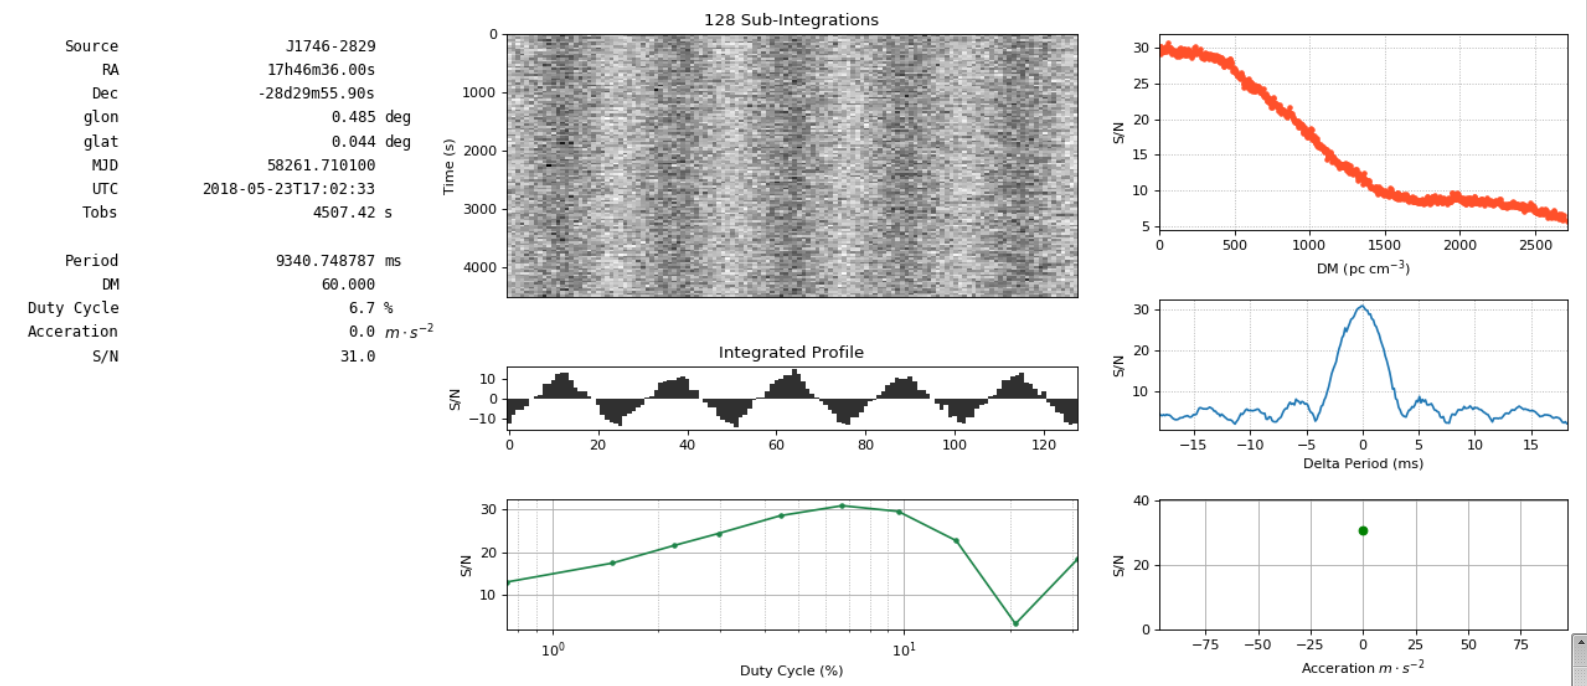
\includegraphics[width=1.0\textwidth]{figures/RFIP.png}
    \label{RFI_p}
    }
\end{figure}
	
\chapter{New RFI mitigation technique} \label{RFI}

     \paragraph{} The list of period bins which is contaminated by RFI will be used as ``zap table''. Zap table also called as Birdie list. Zap table is a list of period to be flagged from the data. If the zap table is available before de-dispersion step, period bins in zap table can be flagged by flagging corresponding period. The flagging is done by apply the FFT to a time series and flag the contaminating period bin. Then, the transformed time series will is applied by invest FFT. The result from this process is flagged data ready to be searched for pulsars. Moreover, zap table can be used in the candidate selections process by ignore candidates with period bins similar to the RFI. As a result, zap table need to be avilable before the searching. In this chapter, I will present a new method to obtain zap list before the observation.
     
     \paragraph{} Since RFI creates numerous artificial pulsar candidates. The number distribution of pulsar candidates from each day of observation over the detected period is studied. Strong periodic RFI will make period bins corresponding to the period of RFI have a large number of candidates. As a result, the periodic RFI is identified by searching for period bins with a high number of candidates. This list of RFI can be used for reprocessing of the data to reduces the number of artificial candidates making the pipeline faster. Also, the distribution of candidates over a long campaign of observation allows us to study the long time behaviour of RFI. 

     \section{RFI mitigation from residual between full dataset and mean}
    \paragraph{} Over 70 million pulsar candidates detected in the FFT pipeline that were observed in HTRU-N pulsar survey is used in this work. More detail about the HTRU pulsar survey will be shown in Section ~\ref{survey}.  This dataset contains 193 days of observations ranging from 21$^{st}$  July 2011 to 30$^{th}$ December 2016. The histogram of pulsar candidates distribution over periods for each observation date is made as Figure ~\ref{RFI_II}. The number distribution of pulsar candidates is normalised by the total number of candidates on the same day to provide the bias from the difference of the observation in each day.
    \paragraph{} First, the ``RFI profile'' is created by calculating the mean of the RFI for each period and subtract that from the full histogram mentioned before as Figure ~\ref{RFI_profile}. The residual is shown in Figure ~\ref{RFI_I}. However, this method detects only dynamics RFI because the ``RFI profile'' is created from the mean of RFI in each period which is already included static RFI. This method shows that the telescope has dynamics RFI. However, since the pulse baseline in the  ``RFI profile'' is not flat especially on short period bins. Consequence with flagging too much data in the short period. In this work, I try to flag as less period bin as possible to avoid accidentally flagging real pulsars. 

\begin{figure}[h!] 
\centering
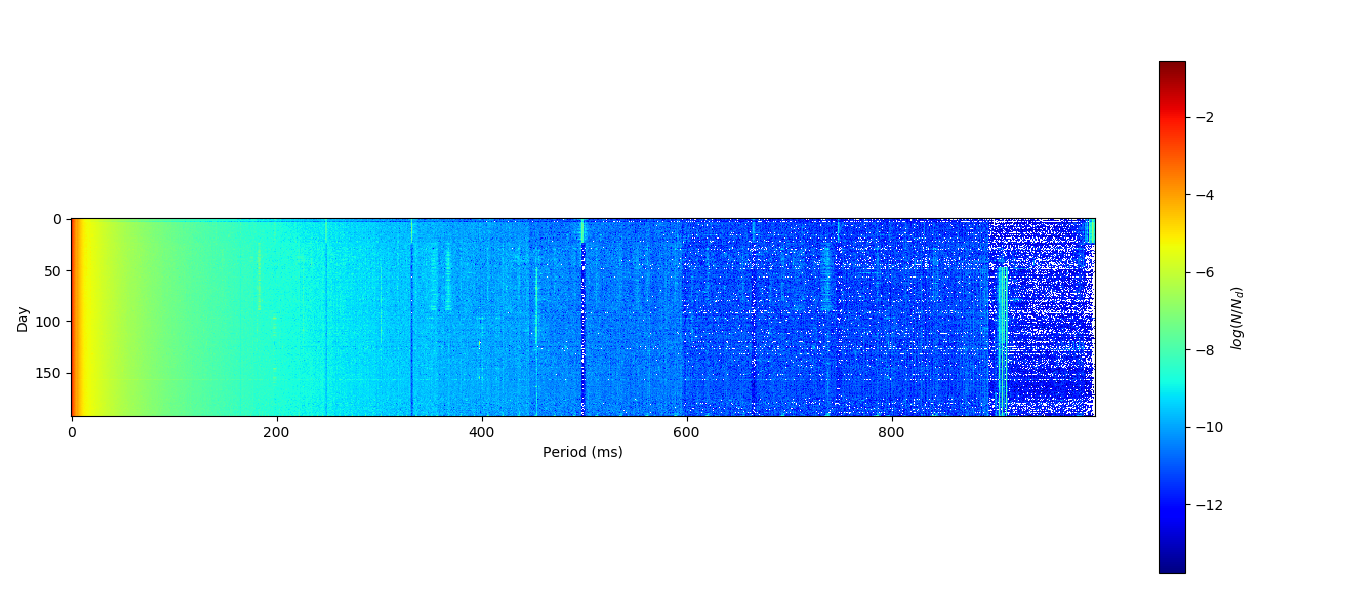
\includegraphics[width=1.0\textwidth]{figures/Full_log.png}
\caption{Distribution of the number of pulsar candidates with the detected period on each observation day. The data is normalised with the total number of candidates on the same day.}
\label{RFI_II}
\end{figure}

\begin{figure}[h!] 
\centering
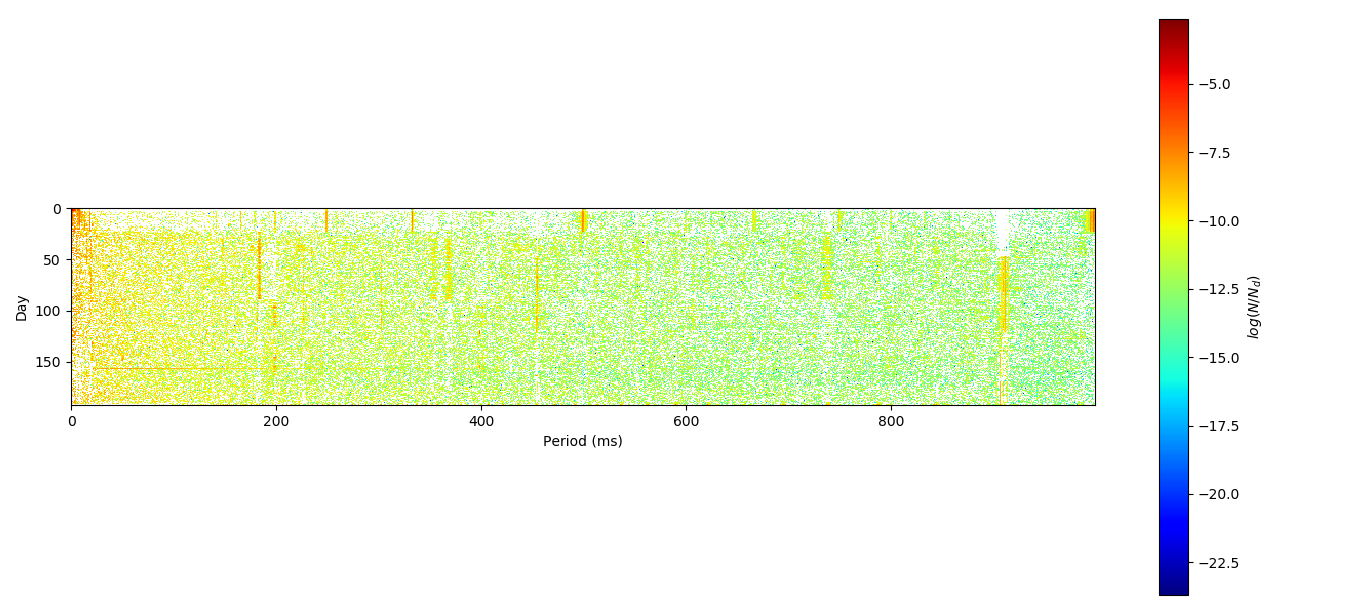
\includegraphics[width=1.0\textwidth]{figures/RFI_mit.png}
\caption{The residual between ~\ref{RFI_II} and ``RFI profile'' }
\label{RFI_I}
\end{figure}

\begin{figure}[h!] 
\centering
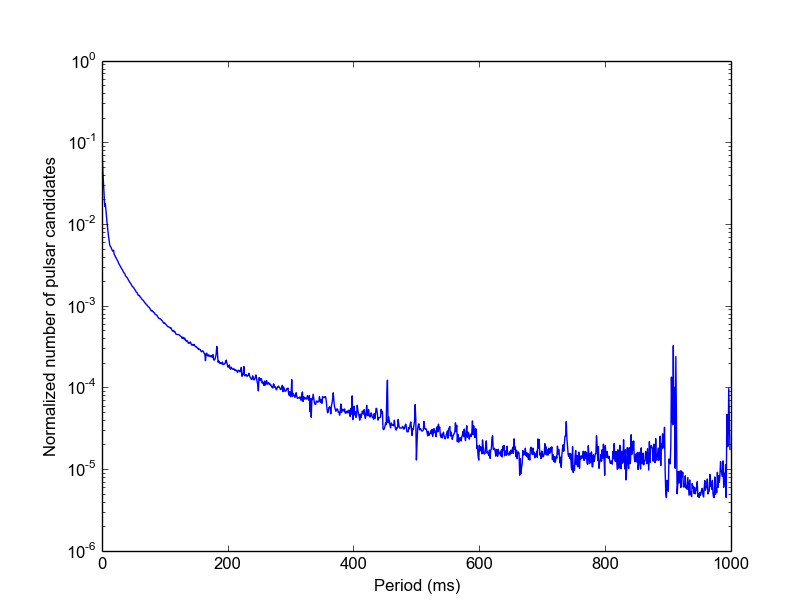
\includegraphics[width=0.7\textwidth]{figures/mean_profile.png}
\caption{"RFI profile" created from an average normalised number of candidates from the whole observation campaign.}
\label{RFI_profile}
\end{figure}

    \section{RFI mitigation from statistic distribution of RFI on each day}
    \paragraph{} On the data that have no periodic RFI, the distribution of pulsar candidates is assumed to be Gaussian distribution. Using the same data set from previous the section, periodic RFI is identified by detecting and flagging period bins that the number of candidates in that bins do not follow the Gaussian distribution. To test how the distribution is similar to the Gaussian distribution. The ``possibility ratio'' between amplitude at percentile corresponding to $3\sigma$ which is 99.730\% is calculated. If the data follows the Gaussian distribution, ratios between each amplitude percentiles and the corresponding standard deviation are unity. This process will be applied repeatedly to the histogram until it follows Gaussian distribution or different between possibility ratio each iteration step is almost constant.
    \paragraph{} By apply this method to the data on each day. The strong periodic RFI is detected. In this work, the only period range from 200ms - 1000ms is used because the ``'RFI profile' getting flat when the period is more than 200ms. The flat profile is needed to avoid flagging all of the short period candidates. Results agree well with the previous section with only $\sim$ 5 $\%$ of the data flagged. The result of this method is shown at ~\ref{RFI_III}. RFI lists from this method are generated and will be tested with previous HTRU-N data in the future. 
 
\begin{figure}[h!] 
\centering
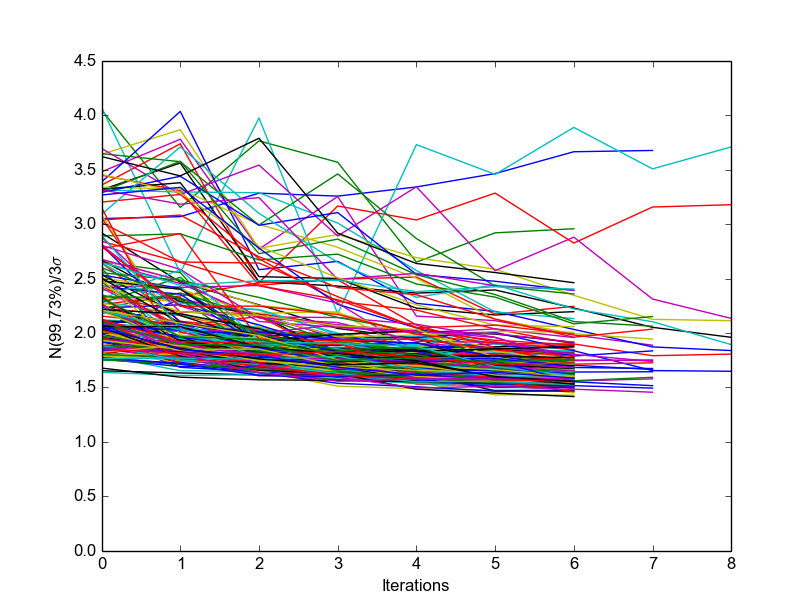
\includegraphics[width=0.7\textwidth]{figures/3sig.png}
\caption{Relation between possibility ratio and iteration for each day. The result shows that most of the data possibility ratio convert to constant number approximately $~\sim$ 2. This implies that the pulsar candidates distribution is not perfectly Gaussian distribution. There are a few days that the ratio are not converted which will be studied carefully in the future.}
\label{RFI_3sig}
\end{figure}

\begin{figure}[h!] 
\centering
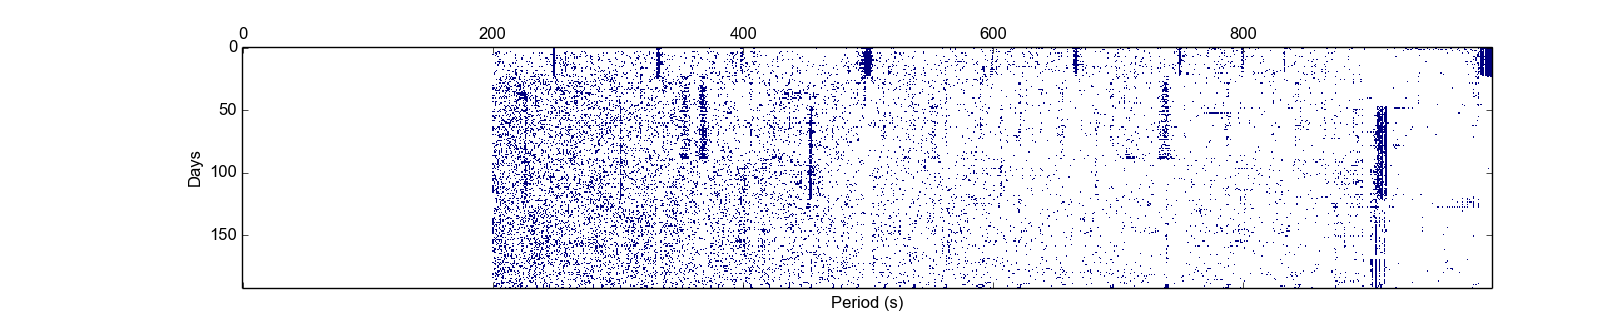
\includegraphics[width=1.0\textwidth]{figures/method2.png}
\caption{Flagged period bins in each day of observation shows the similar result as previous method.}
\label{RFI_III}
\end{figure}
 
 \section{Overview of periodic RFI at Effelsberg telescope }
 \paragraph{} The data shows that the telescope has some RFI in a different epoch. As shown in ~\ref{RFI_II}, the most prominence RFI has a period of$~\sim$ 900ms appeared from day 50 until the end of the observation. Moreover, from day 0-25 which corresponding to 21$^{st}$  July 2011 to 2$^{nd}$  January 2012. There are period bins with high candidates numbers at $~\sim$ 1000, 500, 250 ms and its harmonics. Lastly, period bins around 750 ms and its harmonics appear from days 24 to 89 which corresponding to around 28$^{th}$ February 2012 to 30$^{th}$  December 2014.  
    
     




\end{document}